\documentclass[12pt, a4paper]{article}

% Pacotes
\usepackage[utf8]{inputenc}
\usepackage[T1]{fontenc}
\usepackage[brazil]{babel}
\usepackage{amsmath, amssymb}
\usepackage{graphicx}
\usepackage{booktabs}
\usepackage{multirow}
\usepackage{geometry}
\usepackage{hyperref}
\usepackage{listings}
\usepackage{xcolor}
\usepackage{float}
\usepackage{caption}
\usepackage{subcaption}
\usepackage{array}
\usepackage{enumitem}

\geometry{margin=2.5cm}

\hypersetup{
    colorlinks=true,
    linkcolor=blue,
    urlcolor=blue,
    citecolor=blue
}

\lstset{
    language=Python,
    basicstyle=\ttfamily\footnotesize,
    keywordstyle=\color{blue}\bfseries,
    stringstyle=\color{red},
    commentstyle=\color{gray}\itshape,
    numbers=left,
    numberstyle=\tiny\color{gray},
    frame=single,
    breaklines=true,
    showstringspaces=false,
    tabsize=4
}

\title{%
    \textbf{Relatório de Visão Computacional} \\[0.5cm]
    \large Classificação de Células Cervicais para Detecção de Lesões \\
    Pré-Cancerosas Utilizando YOLOv8
}
\author{Marcelo de Araújo \\ \href{https://github.com/AIWASS23/cte-vc}{Repositório do Projeto}}
\date{\today}

\begin{document}

\maketitle
\tableofcontents
\newpage

% ============================================================
\section{Introdução}
% ============================================================

O presente trabalho aborda um problema de visão computacional que consiste na \textbf{classificação automática de imagens de células cervicais} provenientes do exame de Papanicolaou. O objetivo principal é auxiliar na detecção de lesões pré-cancerosas e cancerosas do colo do útero por meio de técnicas de aprendizado profundo.

O câncer de colo do útero constitui uma das principais causa de óbito por neoplasias malignas entre mulheres em escala global. O exame citopatológico de Papanicolaou é o método de triagem mais amplamente utilizado na prática clínica, entretanto a análise manual das lâminas caracteriza-se por ser um processo demorado e sujeito a variabilidade inter-observador. A automação deste processo através de modelos de aprendizado profundo possibilita aumentar tanto a velocidade quanto a consistência dos diagnósticos.

Neste projeto, foi utilizado o modelo \textbf{YOLOv8} (\textit{You Only Look Once}, versão 8) da Ultralytics no modo de classificação de imagens (\textit{classify}). Embora o YOLO seja tradicionalmente reconhecido como um detector de objetos em tempo real, a versão 8 incorpora um módulo de classificação que permite o seu emprego como classificador de imagens, constituindo uma alternativa as redes convolucionais tradicionais.

\subsection{Objetivos}

Foram definidos dois objetivos complementares para o projeto:

\begin{enumerate}
    \item \textbf{Classificação binária:} Distinguir entre células \textit{Normais} e \textit{Anormais}, proporcionando uma triagem inicial rápida para encaminhamento clínico.
    \item \textbf{Classificação multiclasse:} Classificar as células em 6 categorias diagnósticas específicas --- Negativa, ASC-US, LSIL, ASC-H, HSIL e Carcinoma --- permitindo a identificação do tipo exato da lesão celular.
\end{enumerate}

% ============================================================
\section{Conjunto de Dados}
% ============================================================

\subsection{Origem e Obtenção}

O conjunto de dados utilizado neste trabalho são composto por imagens de células cervicais no formato TIFF (\textit{Tagged Image File Format}), obtidas a partir de exames citopatológicos de Papanicolaou. As imagens possuem dimensões de $50 \times 50$ pixels em 3 canais de cor (RGB).

\textbf{Fonte do dataset:} O conjunto de imagens foi fornecido diretamente por um professor da universidade, sendo composto por amostras citológicas cervicais organizadas e rotuladas para fins didáticos e de pesquisa acadêmica.

\subsection{Estrutura e Distribuição}

O dataset encontra-se organizado em subpastas dentro do diretório \texttt{cells/}, onde cada subpasta corresponde a uma categoria diagnóstica conforme o Sistema Bethesda para classificação citológica cervical. A Tabela~\ref{tab:distribuicao} apresenta a distribuição completa das amostras.

\begin{table}[H]
\centering
\caption{Distribuição das classes no dataset utilizado.}
\label{tab:distribuicao}
\begin{tabular}{llcl}
\toprule
\textbf{Subpasta} & \textbf{Diagnóstico} & \textbf{Imagens} & \textbf{Classe Binária} \\
\midrule
Negativa  & Negativo para lesão intraepitelial               & 5.500 & Normal  \\
ASC-US    & Cél. escamosas atípicas de signif. indeterminado & 620   & Anormal \\
LSIL      & Lesão intraepitelial escamosa de baixo grau      & 1.300 & Anormal \\
ASC-H     & Cél. escamosas atípicas, não excluindo HSIL      & 910   & Anormal \\
HSIL      & Lesão intraepitelial escamosa de alto grau        & 1.680 & Anormal \\
Carcinoma & Carcinoma de células escamosas                    & 120   & Anormal \\
\midrule
\multicolumn{2}{l}{\textbf{Total}} & \textbf{10.130} & --- \\
\bottomrule
\end{tabular}
\end{table}

Observa-se a presença de um \textbf{desbalanceamento significativo} entre as classes. A classe Negativa concentra 54,3\% do total de amostras, enquanto a classe Carcinoma representa apenas 1,2\% do conjunto. Este cenário é condizente com a distribuição esperada em contextos clínicos reais, onde casos normais são majoritários.

\subsection{Pré-processamento e Organização para YOLOv8}

O modelo YOLOv8 no modo \textit{classify} requer que os dados estejam organizados em uma estrutura hierárquica de diretórios com subpastas \texttt{train/} e \texttt{val/}. Desta forma, o pré-processamento envolveram as seguintes etapas:

\begin{enumerate}
    \item \textbf{Coleta dos caminhos:} Todos os arquivos de imagem (\texttt{.tif}) foram percorridos recursivamente nas subpastas do diretório \texttt{cells/}, associando cada imagem ao rótulo correspondente da sua subpasta de origem.

    \item \textbf{Divisão estratificada:} O conjunto foi particionado em treino (80\%) e validação (20\%) utilizando a função \texttt{train\_test\_split} do scikit-learn com os parâmetros \texttt{random\_state=42} e \texttt{stratify=labels}, garantindo que a proporção de cada classe fosse mantido em ambos os subconjuntos.

    \item \textbf{Reorganização dos diretórios:} As imagens foram copiadas para a nova estrutura de pastas exigida pelo YOLOv8:
\end{enumerate}

Para a classificação \textbf{binária}, as 6 subpastas originais foram agrupadas em duas classes:
\begin{verbatim}
    dataset_yolo_binario/
    ├── train/
    │   ├── Normal/      (imagens da subpasta Negativa)
    │   └── Anormal/     (imagens de ASC-US, LSIL, ASC-H, HSIL, carcinoma)
    └── val/
        ├── Normal/
        └── Anormal/
\end{verbatim}

Para a classificação \textbf{multiclasse}, cada subpasta original foi preservada:
\begin{verbatim}
    dataset_yolo_doencas/
    ├── train/
    │   ├── ASC-H/  ├── ASC-US/  ├── HSIL/
    │   ├── LSIL/   ├── Negativa/  └── carcinoma/
    └── val/
        └── (mesmas 6 subpastas)
\end{verbatim}

A normalização das imagens e o redimensionamento são realizadas automaticamente pelo YOLOv8 durante o treinamento, não necessitando de tratamento manual.

\subsection{Divisão dos Dados}

\begin{table}[H]
\centering
\caption{Divisão do dataset em treinamento e validação.}
\label{tab:divisao}
\begin{tabular}{lcc}
\toprule
\textbf{Conjunto} & \textbf{Proporção} & \textbf{Imagens (aprox.)} \\
\midrule
Treinamento & 80\% & 8.104 \\
Validação   & 20\% & 2.026 \\
\midrule
\textbf{Total} & 100\% & 10.130 \\
\bottomrule
\end{tabular}
\end{table}

% ============================================================
\section{Fluxo Completo da Solução}
% ============================================================

A Figura~\ref{fig:fluxo} apresenta o diagrama esquemático do fluxo completo implementado neste trabalho, aplicável a ambos os experimentos (binário e multiclasse).

\begin{figure}[H]
\centering
\fbox{
\begin{minipage}{0.85\textwidth}
\centering
\vspace{0.3cm}
\textbf{FLUXO DA SOLUÇÃO --- YOLOv8 Classify} \\[0.3cm]
\begin{tabular}{c}
\fbox{1. Dataset original (\texttt{cells/} --- 6 subpastas por doença)} \\
$\downarrow$ \\
\fbox{2. Coleta de caminhos e rótulos (\texttt{os.walk})} \\
$\downarrow$ \\
\fbox{3. Divisão estratificada 80/20 (\texttt{train\_test\_split}, stratify)} \\
$\downarrow$ \\
\fbox{4. Reorganização em \texttt{train/} e \texttt{val/} (cópia de arquivos)} \\
$\downarrow$ \\
\fbox{5. Carregamento do modelo pré-treinado (\texttt{yolov8n-cls.pt})} \\
$\downarrow$ \\
\fbox{6. Treinamento com \textit{fine-tuning} (10 épocas, batch 32, imgsz 50)} \\
$\downarrow$ \\
\fbox{7. Inferência sobre conjunto de validação (\texttt{model.predict})} \\
$\downarrow$ \\
\fbox{8. Cálculo de métricas (Acurácia, Precisão, Recall, F1, Especificidade)} \\
$\downarrow$ \\
\fbox{9. Geração de gráficos e matrizes de confusão} \\
\end{tabular}
\vspace{0.3cm}
\end{minipage}
}
\caption{Fluxo completo da solução proposta utilizando YOLOv8 no modo \textit{classify}.}
\label{fig:fluxo}
\end{figure}

% ============================================================
\section{Arquitetura do Modelo: YOLOv8 Classify}
% ============================================================

O YOLO (\textit{You Only Look Once}) é uma família de modelos de aprendizado profundo originalmente projetados para detecção de objetos em tempo real. A versão 8, desenvolvida pela Ultralytics, expandiu as capacidades do framework para incluir tarefas de \textbf{classificação de imagens}, além da detecção e segmentação. Esta seção detalham o funcionamento do YOLOv8 no modo \textit{classify}, uma vez que esta abordagem não é tipicamente abordada em disciplinas convencionais de visão computacional.

\subsection{Backbone: CSPDarknet}

O extrator de características (\textit{backbone}) do YOLOv8 é baseado em uma versão modificada do \textbf{CSPDarknet} (\textit{Cross-Stage Partial Darknet}). Diferentemente de uma CNN sequencial simples, o CSPDarknet emprega conexões parciais entre estágios (\textit{Cross-Stage Partial connections}), que dividem o fluxo de gradientes em dois caminhos distintos. Esta estratégia reduz a redundância computacional e melhora o aprendizado de características, permitindo que a rede aprenda representações mais rica com menos parâmetros.

O backbone aplica sucessivas operações de \textbf{convolução}, \textbf{normalização por lote} (\textit{batch normalization}) e ativação \textbf{SiLU} (\textit{Sigmoid Linear Unit}):

\begin{equation}
    \text{SiLU}(x) = x \cdot \sigma(x) = \frac{x}{1 + e^{-x}}
\end{equation}

onde $\sigma(x)$ é a função sigmoide. A SiLU é uma função de ativação suave e não-monótona que tende a apresentar melhor desempenho que a ReLU em redes profundas.

\subsection{Classificador}

Após a extração de características pelo backbone, o módulo de classificação do YOLOv8 aplica:

\begin{enumerate}
    \item \textbf{Global Average Pooling (GAP):} Reduz cada mapa de características a um único valor escalar, calculando a média de todos os elementos espaciais:
    \begin{equation}
        z_k = \frac{1}{H \times W} \sum_{i=1}^{H} \sum_{j=1}^{W} f_k(i, j)
    \end{equation}
    onde $f_k(i,j)$ é o valor do $k$-ésimo mapa de características na posição $(i,j)$, e $H \times W$ são as dimensões espaciais.

    \item \textbf{Camada Linear (\textit{Fully Connected}):} Mapeia o vetor de características para o espaço de $K$ classes, produzindo os logits de saída.

    \item \textbf{Softmax:} Converte os logits em probabilidades normalizadas:
    \begin{equation}
        P(y = c \mid \mathbf{x}) = \frac{e^{z_c}}{\sum_{j=1}^{K} e^{z_j}}
    \end{equation}
\end{enumerate}

\subsection{\textit{Transfer Learning}}

Uma das principais vantagem do YOLOv8 em relação a CNNs construídas do zero é a utilização de \textbf{\textit{transfer learning}} (aprendizado por transferência). O modelo base \texttt{yolov8n-cls.pt} (variante \textit{nano}) é disponibilizado com pesos pré-treinados no dataset \textbf{ImageNet}, que contém aproximadamente 1,2 milhão de imagens distribuídas em 1.000 classes.

O processo de \textit{transfer learning} consiste em:

\begin{enumerate}
    \item Carregar os pesos pré-treinados, que já codificam conhecimento sobre extração de bordas, texturas, formas e padrões visuais genéricos.
    \item Substituir a camada de classificação final para adequar o número de saídas ao problema específico (2 classes no binário, 6 no multiclasse).
    \item Realizar o \textit{fine-tuning} (ajuste fino) dos pesos em todo o modelo utilizando o dataset de células cervicais.
\end{enumerate}

Esta abordagem é particularmente vantajosa para datasets de tamanho reduzido ou com desbalanceamento entre classes, pois os pesos iniciais já possuem uma boa representação de características visual de baixo e médio nível.

\subsection{Parâmetros de Treinamento}

A Tabela abaixo resume os hiperparâmetros utilizados nos experimentos de treinamento.

\begin{table}[H]
\centering
\caption{Hiperparâmetros de treinamento do YOLOv8.}
\label{tab:parametros}
\begin{tabular}{ll}
\toprule
\textbf{Parâmetro} & \textbf{Valor} \\
\midrule
Modelo base            & \texttt{yolov8n-cls.pt} (nano) \\
Tamanho da imagem      & $50 \times 50$ pixels \\
Épocas                 & 10 \\
Tamanho do \textit{batch}  & 32 \\
Dispositivo            & Apple MPS (Metal Performance Shaders) \\
Otimizador             & SGD com momentum (padrão Ultralytics) \\
Função de perda        & Cross-Entropy \\
Validação por época    & Sim (\texttt{val=True}) \\
Pesos iniciais         & Pré-treinados no ImageNet \\
\bottomrule
\end{tabular}
\end{table}

% ============================================================
\section{Métricas de Avaliação}
% ============================================================

Para avaliar quantitativamente o desempenho dos modelos, foram empregadas as métricas descritas a seguir. Todas as métricas foram calculados utilizando a biblioteca scikit-learn a partir das predições do modelo sobre o conjunto de validação.

\subsection{Acurácia}

A acurácia corresponde à proporção de predições corretas em relação ao total de amostras avaliadas:

\begin{equation}
    \text{Acurácia} = \frac{VP + VN}{VP + VN + FP + FN}
\end{equation}

onde $VP$ = verdadeiros positivos, $VN$ = verdadeiros negativos, $FP$ = falsos positivos e $FN$ = falsos negativos.

\subsection{Precisão}

A precisão (\textit{precision}) quantifica a proporção de verdadeiros positivos dentre todas as predições positivas realizadas pelo modelo:

\begin{equation}
    \text{Precisão} = \frac{VP}{VP + FP}
\end{equation}

\subsection{Revocação (Sensibilidade)}

A revocação (\textit{recall}) mede a capacidade do modelo de identificar corretamente todas as amostras positivas:

\begin{equation}
    \text{Revocação} = \frac{VP}{VP + FN}
\end{equation}

No contexto clínico, a revocação é particularmente relevante, pois um falso negativo (lesão não detectada) pode ter consequências graves para a paciente.

\subsection{F1-Score}

O F1-Score constitui a média harmônica entre a precisão e a revocação, fornecendo uma medida balanceada entre ambas:

\begin{equation}
    F_1 = 2 \cdot \frac{\text{Precisão} \times \text{Revocação}}{\text{Precisão} + \text{Revocação}}
\end{equation}

Na avaliação multiclasse, foi utilizada a versão \textit{weighted}, na qual o F1-Score de cada classe é ponderada pelo número de amostras daquela classe:

\begin{equation}
    F_{1,\text{weighted}} = \sum_{c=1}^{K} \frac{n_c}{N} \cdot F_{1,c}
\end{equation}

onde $n_c$ é o número de amostras da classe $c$ e $N$ o total de amostras.

\subsection{Especificidade}

A especificidade avalia a capacidade do modelo em identificar corretamente as amostras negativas:

\begin{equation}
    \text{Especificidade} = \frac{VN}{VN + FP}
\end{equation}

Para o cenário multiclasse, a especificidade foram calculada individualmente para cada classe $c$ utilizando a abordagem \textit{one-vs-rest}:

\begin{equation}
    \text{Especificidade}_c = \frac{VN_c}{VN_c + FP_c}
\end{equation}

onde $VN_c = \sum_{i \neq c}\sum_{j \neq c} M_{i,j}$ e $FP_c = \sum_{i \neq c} M_{i,c}$, sendo $M$ a matriz de confusão.

\subsection{Matriz de Confusão}

A matriz de confusão $M$ de dimensão $K \times K$ sumariza a distribuição das predições em relação aos rótulos verdadeiros. O elemento $M_{i,j}$ indica a quantidade de amostras pertencentes à classe $i$ que foi classificada como pertencente à classe $j$. Os elementos na diagonal principal ($M_{i,i}$) representam as classificações corretas.

% ============================================================
\section{Ajuste de Hiperparâmetros}
% ============================================================

O ajuste de hiperparâmetros foi conduzido de forma sistemática, variando individualmente quatro hiperparâmetros distintos --- número de épocas, tamanho do \textit{batch}, taxa de aprendizado e variante do modelo --- enquanto os demais permaneciam fixos. Esta abordagem de variação controlada permite isolar o efeito de cada hiperparâmetro sobre o desempenho do modelo. Os experimentos foram executados tanto para a classificação binária quanto para a multiclasse.

\subsection{Experimentos Realizados}

A Tabela abixo apresenta a configuração completa dos 8 experimentos conduzidos para cada cenário de classificação:

\begin{table}[H]
\centering
\caption{Configuração dos experimentos de variação de hiperparâmetros.}
\label{tab:experimentos}
\begin{tabular}{lccccc}
\toprule
\textbf{Experimento} & \textbf{Modelo} & \textbf{Épocas} & \textbf{Batch} & \textbf{LR} & \textbf{Variável} \\
\midrule
base       & yolov8n-cls & 10 & 32 & 0,01  & --- (referência) \\
epochs\_5  & yolov8n-cls & 5  & 32 & 0,01  & Épocas \\
epochs\_20 & yolov8n-cls & 20 & 32 & 0,01  & Épocas \\
batch\_16  & yolov8n-cls & 10 & 16 & 0,01  & Batch size \\
batch\_64  & yolov8n-cls & 10 & 64 & 0,01  & Batch size \\
lr\_0001   & yolov8n-cls & 10 & 32 & 0,001 & Learning rate \\
lr\_005    & yolov8n-cls & 10 & 32 & 0,05  & Learning rate \\
modelo\_s  & yolov8s-cls & 10 & 32 & 0,01  & Arquitetura \\
\bottomrule
\end{tabular}
\end{table}

\subsection{Justificativa das Variações}

\begin{itemize}
    \item \textbf{Número de épocas (5, 10, 20):} Avalia se o modelo converge adequadamente com menos treinamento ou se beneficia de épocas adicionais. Um número insuficiente de épocas pode resultar em \textit{underfitting}, enquanto épocas em excesso podem causar \textit{overfitting}.

    \item \textbf{Tamanho do batch (16, 32, 64):} O tamanho do batch afeta a estimativa do gradiente durante o treinamento. Batches menores introduzem mais ruído (efeito regularizador), enquanto batches maiores proporcionam estimativas mais estáveis, mas podem convergir para mínimos locais menos generalizáveis.

    \item \textbf{Taxa de aprendizado (0,001; 0,01; 0,05):} A taxa de aprendizado controla a magnitude das atualizações dos pesos. Valores muito baixos resultam em convergência lenta, enquanto valores muito altos pode causar divergência ou oscilações durante o treinamento.

    \item \textbf{Variante do modelo (nano vs. small):} O YOLOv8n-cls (\textit{nano}) possui menos parâmetros e é mais rápido, enquanto o YOLOv8s-cls (\textit{small}) tem maior capacidade de representação. Esta variação avalia o \textit{trade-off} entre complexidade do modelo e desempenho.
\end{itemize}

\subsection{Resultados da Variação --- Classificação Binária}

A Tabela~\ref{tab:hiper_binario} apresentam os resultados obtidos nos 8 experimentos do cenário binário:

\begin{table}[H]
\centering
\caption{Resultados da variação de hiperparâmetros --- classificação binária.}
\label{tab:hiper_binario}
\begin{tabular}{lccccc}
\toprule
\textbf{Experimento} & \textbf{Acurácia} & \textbf{Precisão} & \textbf{Revocação} & \textbf{F1} & \textbf{Espec.} \\
\midrule
base       & 0.920533 & 0.922160 & 0.920533 & 0.920191 & 0.874730 \\
epochs\_5  & 0.920533 & 0.922160 & 0.920533 & 0.920191 & 0.874730 \\
epochs\_20 & 0.923495 & 0.924847 & 0.923495 & 0.923201 & 0.881210 \\
batch\_16  & 0.919546 & 0.919730 & 0.919546 & 0.919420 & 0.895248 \\
batch\_64  & 0.918559 & 0.919510 & 0.918559 & 0.918294 & 0.880130 \\
lr\_0001   & 0.920533 & 0.922160 & 0.920533 & 0.920191 & 0.874730 \\
lr\_005    & 0.920533 & 0.922160 & 0.920533 & 0.920191 & 0.874730 \\
modelo\_s  & 0.926456 & 0.926561 & 0.926456 & 0.926366 & 0.906048 \\
\bottomrule
\end{tabular}
\end{table}

\textit{Nota: Execute \texttt{yolo\_binario\_hiperparametros.py} para obter os valores. Os resultados também são salvos automaticamente em \texttt{resultados\_hiperparametros\_binario.csv}.}

\begin{figure}[H]
    \centering
    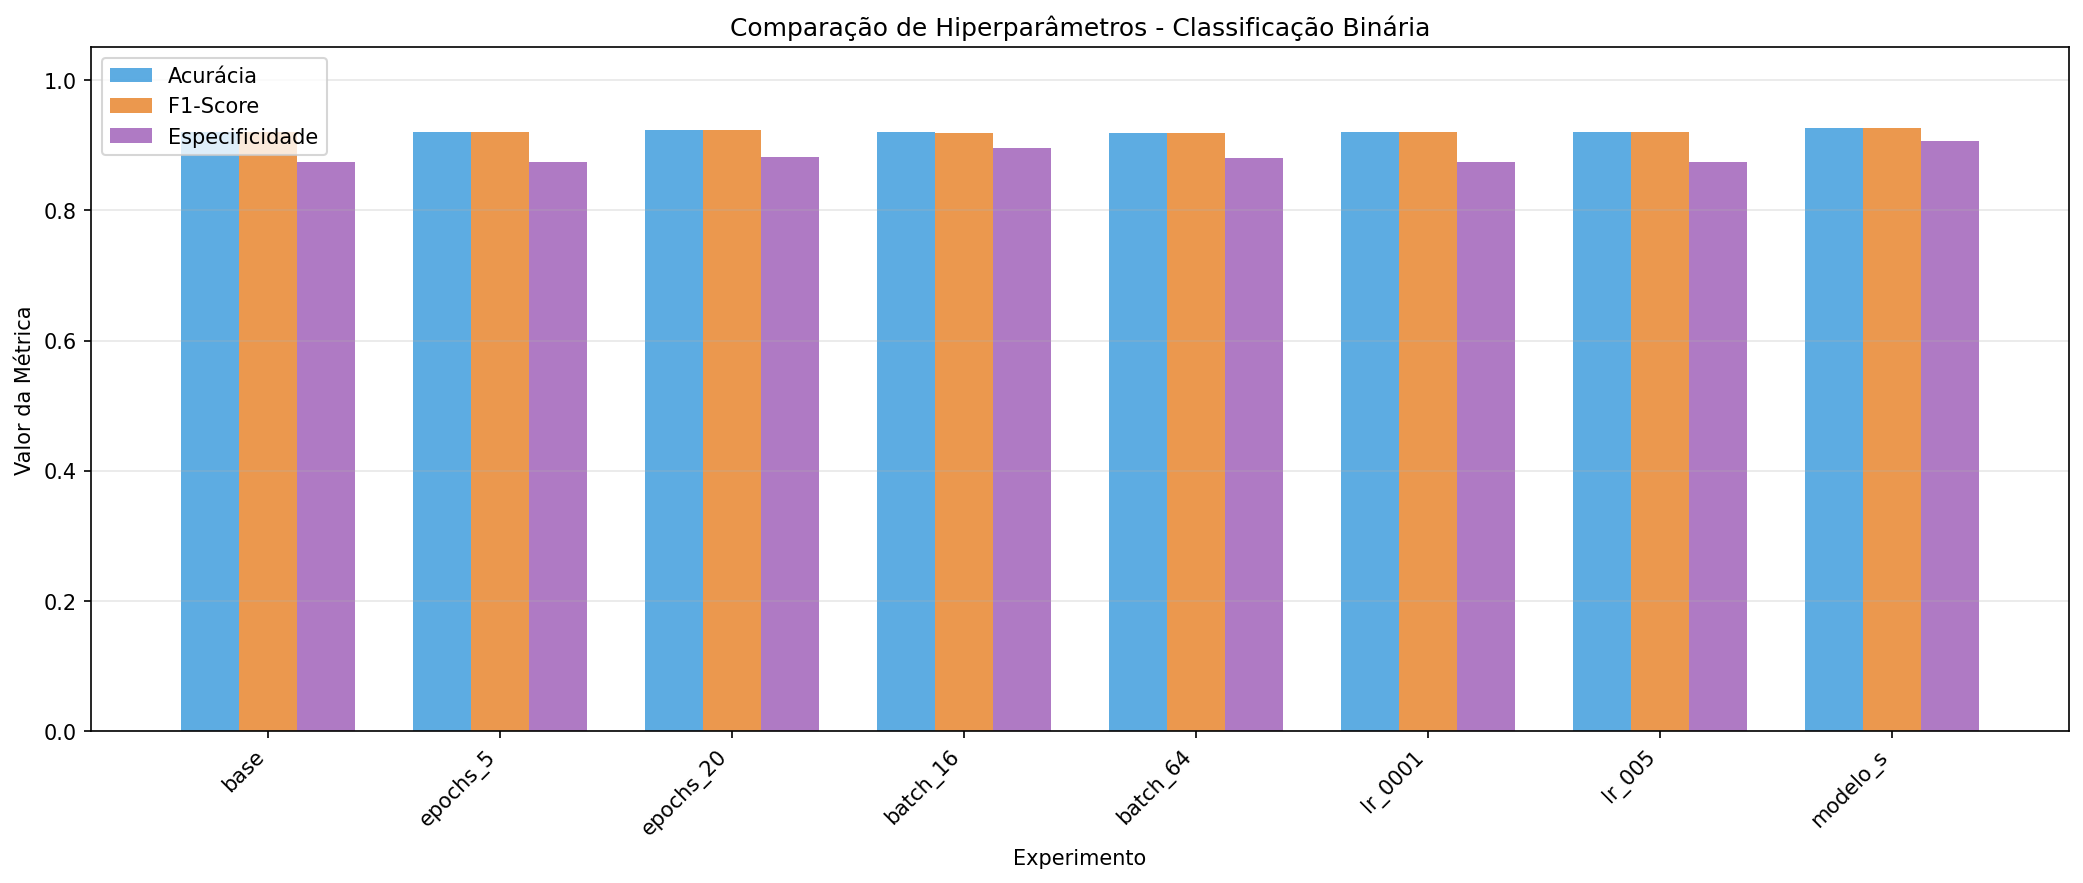
\includegraphics[width=0.95\textwidth]{yolo_binaria_comparacao_hiperparametros.png}
    \caption{Comparação geral dos hiperparâmetros --- classificação binária.}
    \label{fig:hiper_bin_comp}
\end{figure}

\begin{figure}[H]
    \centering
    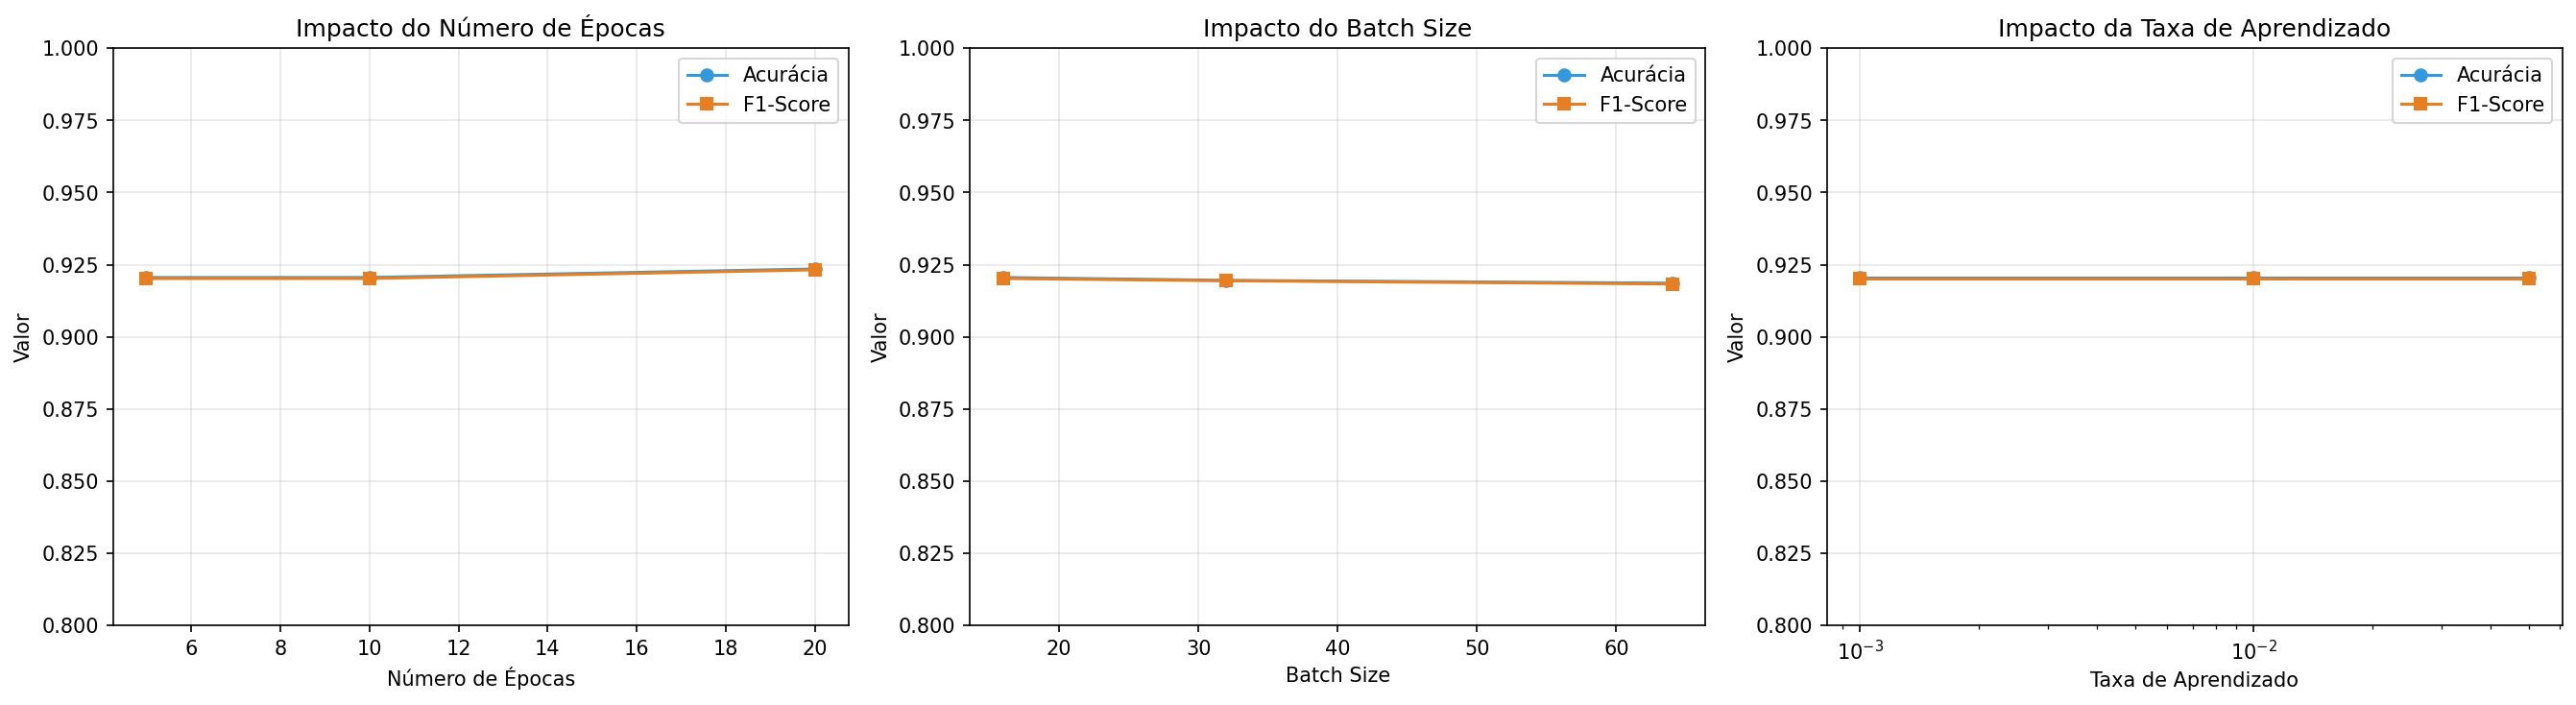
\includegraphics[width=0.95\textwidth]{yolo_binaria_variacao_hiperparametros.png}
    \caption{Impacto individual de cada hiperparâmetro --- classificação binária.}
    \label{fig:hiper_bin_var}
\end{figure}

\subsection{Resultados da Variação --- Classificação Multiclasse}

A Tabela abaixo apresenta os resultados obtidos nos 8 experimentos do cenário multiclasse:

\begin{table}[H]
\centering
\caption{Resultados da variação de hiperparâmetros --- classificação multiclasse.}
\label{tab:hiper_multi}
\begin{tabular}{lccccc}
\toprule
\textbf{Experimento} & \textbf{Acurácia} & \textbf{Precisão} & \textbf{Revocação} & \textbf{F1} & \textbf{Espec. Méd.} \\
\midrule
base       & 0.823791 & 0.810327 & 0.823791 & 0.809436 & 0.950794 \\
epochs\_5  & 0.823791 & 0.810327 & 0.823791 & 0.809436 & 0.950794 \\
epochs\_20 & 0.832182 & 0.818056 & 0.832182 & 0.820760 & 0.955669 \\
batch\_16  & 0.821816 & 0.806538 & 0.821816 & 0.808147 & 0.951873 \\
batch\_64  & 0.829220 & 0.816419 & 0.829220 & 0.816076 & 0.953302 \\
lr\_0001   & 0.823791 & 0.810327 & 0.823791 & 0.809436 & 0.950794 \\
lr\_005    & 0.823791 & 0.810327 & 0.823791 & 0.809436 & 0.950794 \\
modelo\_s  & 0.846002 & 0.834399 & 0.846002 & 0.838300 & 0.961084 \\
\bottomrule
\end{tabular}
\end{table}

\textit{Nota: Execute \texttt{yolo\_doencas\_hiperparametros.py} para obter os valores. Os resultados também são salvos em \texttt{resultados\_hiperparametros\_doencas.csv}.}

\begin{figure}[H]
    \centering
    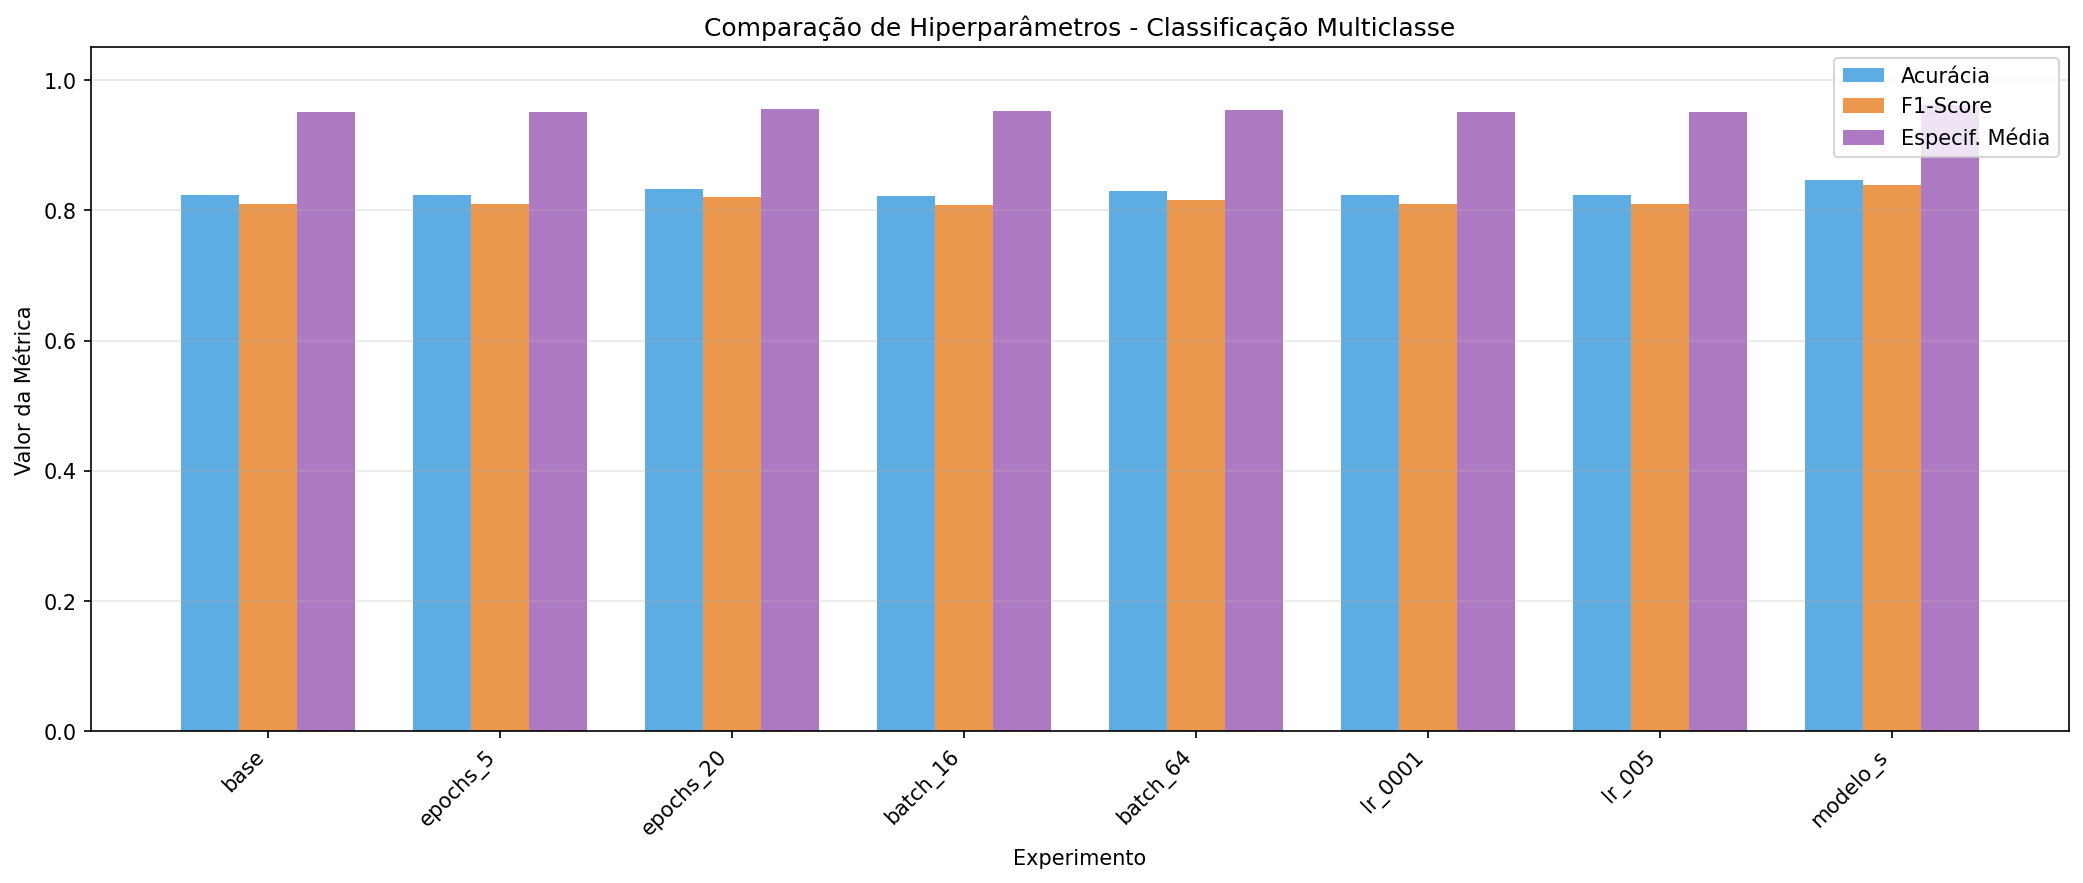
\includegraphics[width=0.95\textwidth]{yolo_multiclasse_comparacao_hiperparametros.png}
    \caption{Comparação geral dos hiperparâmetros --- classificação multiclasse.}
    \label{fig:hiper_multi_comp}
\end{figure}

\begin{figure}[H]
    \centering
    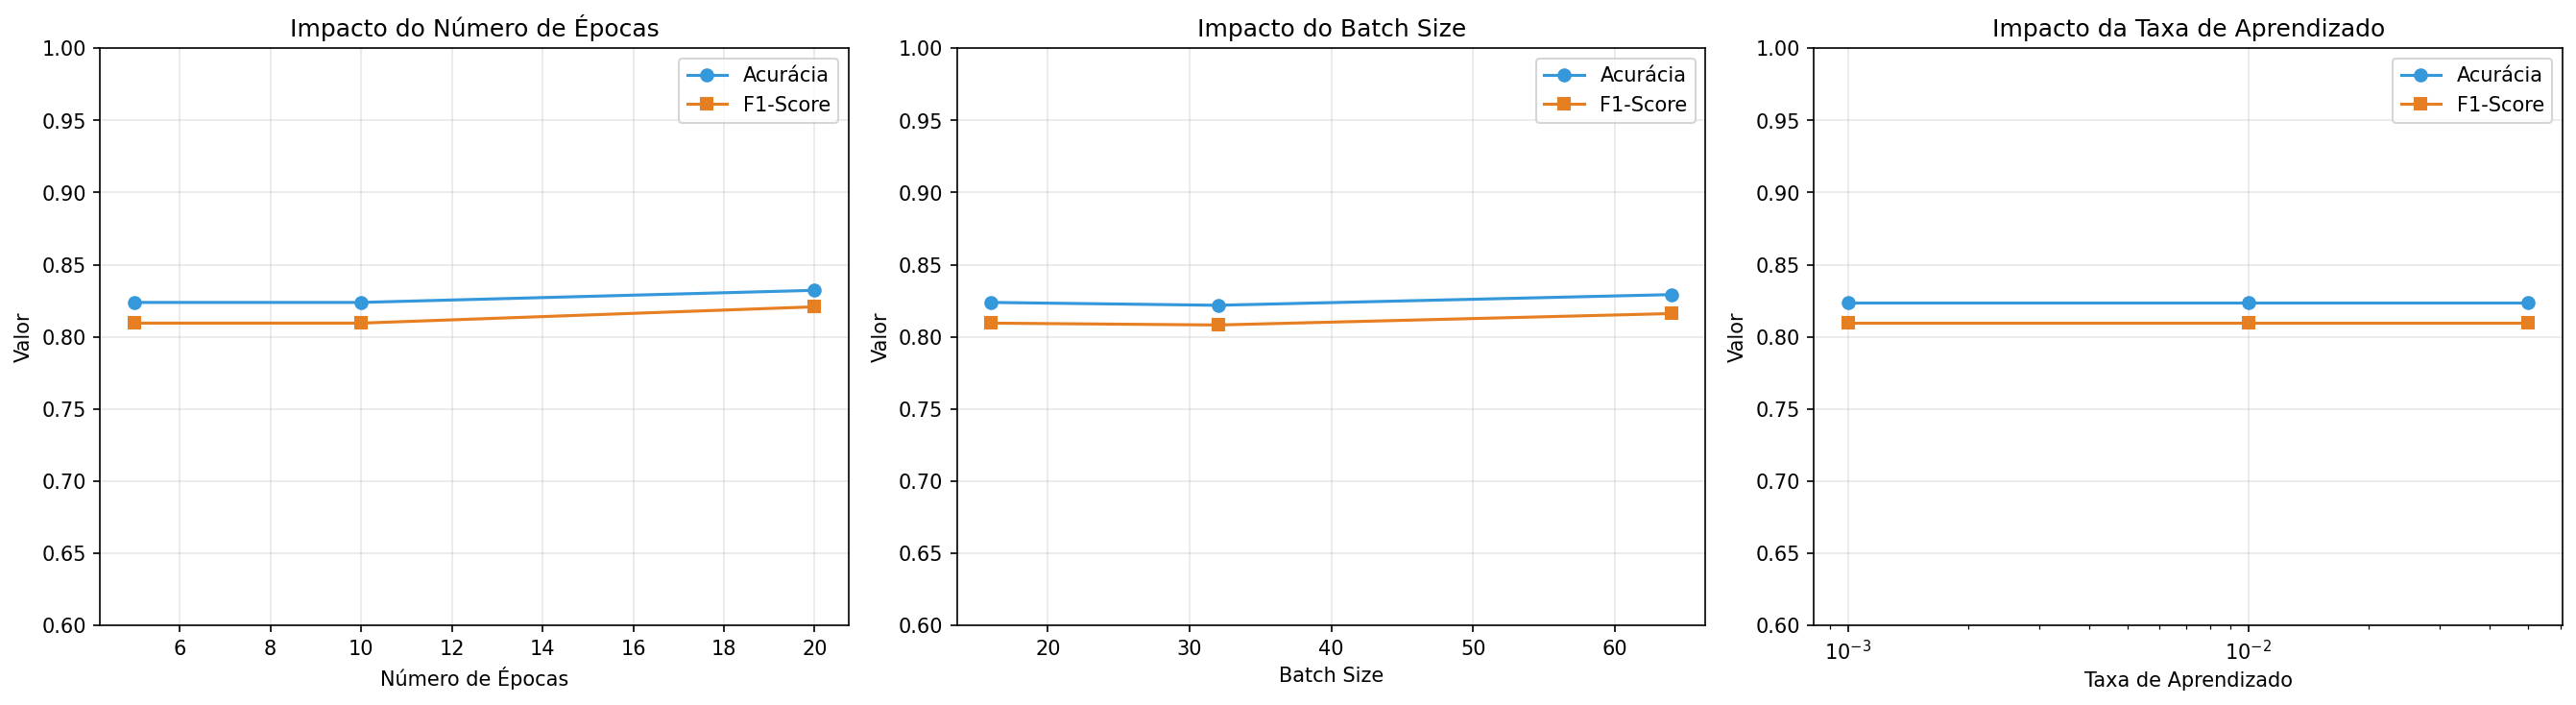
\includegraphics[width=0.95\textwidth]{yolo_multiclasse_variacao_hiperparametros.png}
    \caption{Impacto individual de cada hiperparâmetro --- classificação multiclasse.}
    \label{fig:hiper_multi_var}
\end{figure}

% ============================================================
\section{Resultados} \label{sec:resultados}
% ============================================================

\subsection{Experimento 1: Classificação Binária (Normal vs. Anormal)}

O primeiro experimento consistiu na classificação das células em duas categorias: Normal (correspondendo à subpasta Negativa) e Anormal (agrupando ASC-US, LSIL, ASC-H, HSIL e Carcinoma). A Tabela~\ref{tab:res_binario} apresenta as métricas obtida.

\begin{table}[H]
\centering
\caption{Resultados do modelo YOLOv8 para classificação binária.}
\label{tab:res_binario}
\begin{tabular}{lc}
\toprule
\textbf{Métrica} & \textbf{Valor} \\
\midrule
Acurácia              & 0,9205 \\
Precisão (weighted)   & 0,9222 \\
Revocação (weighted)  & 0,9205 \\
F1-Score (weighted)   & 0,9202 \\
Especificidade        & 0,8747 \\
\bottomrule
\end{tabular}
\end{table}

O modelo atingiu uma acurácia de \textbf{92,05\%}, demonstrando boa capacidade de distinguir entre células normais e anormais. A especificidade de 87,47\% indica que o modelo classifica corretamente a grande maioria das células anormais, embora 12,5\% das amostras anormais sejam erroneamente classificadas como normais (falsos negativos).

A Tabela abaixo apresenta a matriz de confusão obtida:

\begin{table}[H]
\centering
\caption{Matriz de confusão --- classificação binária.}
\label{tab:cm_binario}
\begin{tabular}{lcc}
\toprule
 & \textbf{Pred. Anormal} & \textbf{Pred. Normal} \\
\midrule
\textbf{Real Anormal} & 810  & 116 \\
\textbf{Real Normal}  & 45   & 1.055 \\
\bottomrule
\end{tabular}
\end{table}

Dos 2.026 exemplos do conjunto de validação, 1.865 foram classificados corretamente. Foram observados 116 falsos negativos (amostras anormais classificadas como normais) e 45 falsos positivos (amostras normais classificadas como anormais).

\begin{figure}[H]
    \centering
    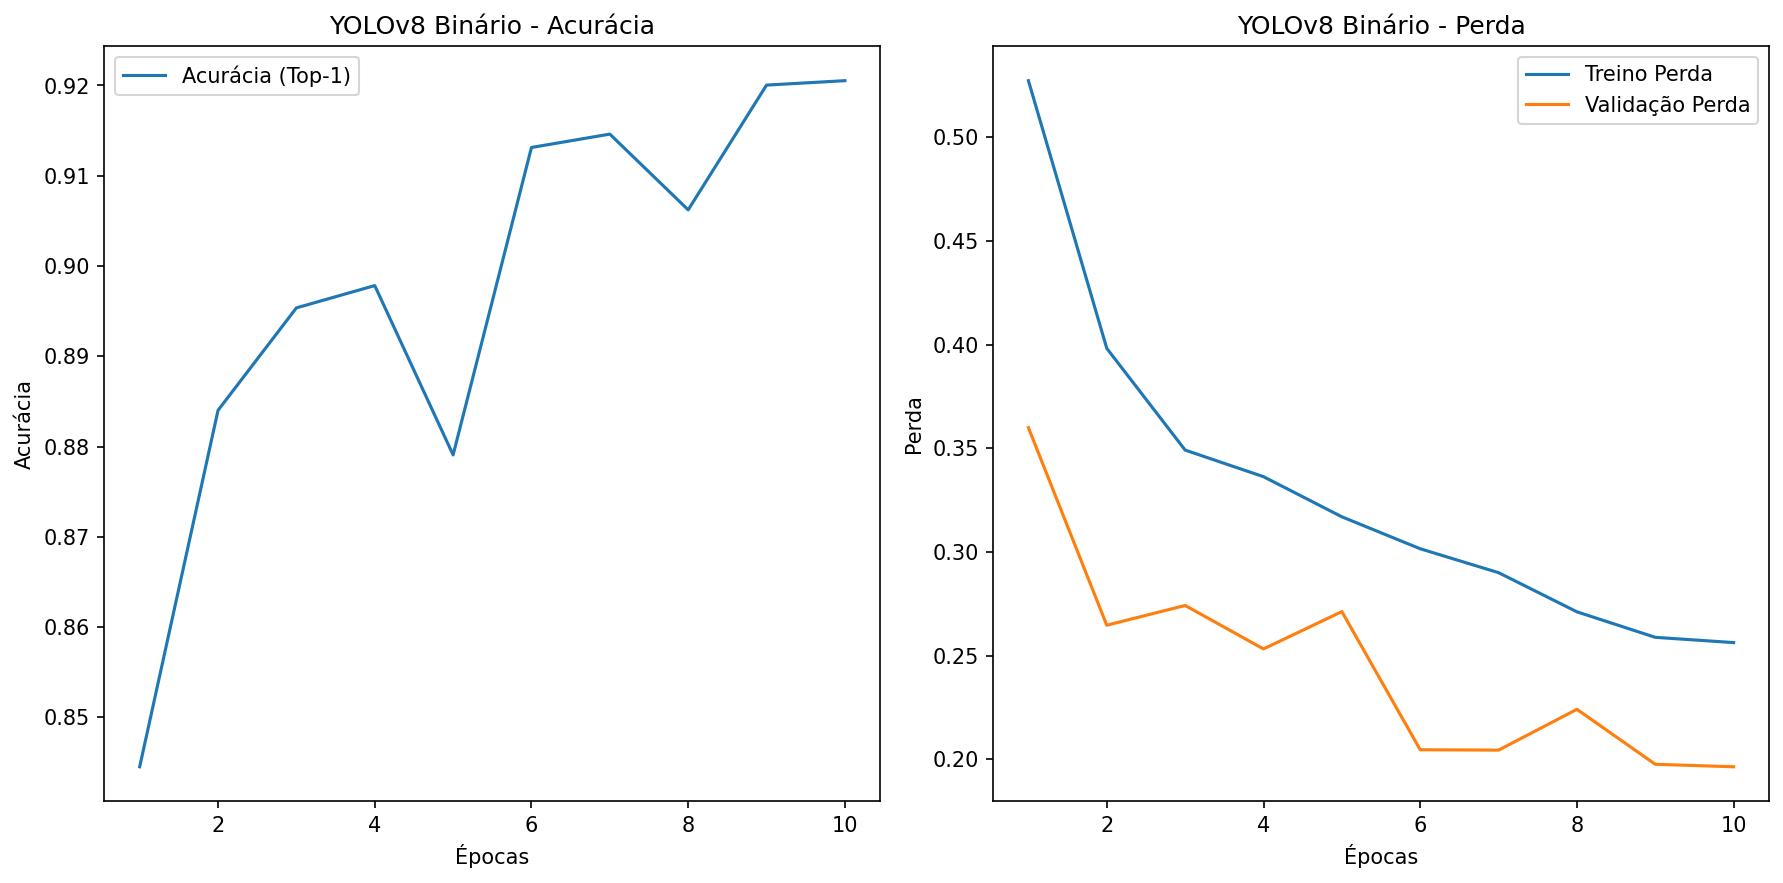
\includegraphics[width=0.9\textwidth]{yolo_binaria_acuracia_perda.png}
    \caption{Curvas de acurácia e perda ao longo das épocas --- classificação binária.}
    \label{fig:ybin_acc_loss}
\end{figure}

\begin{figure}[H]
    \centering
    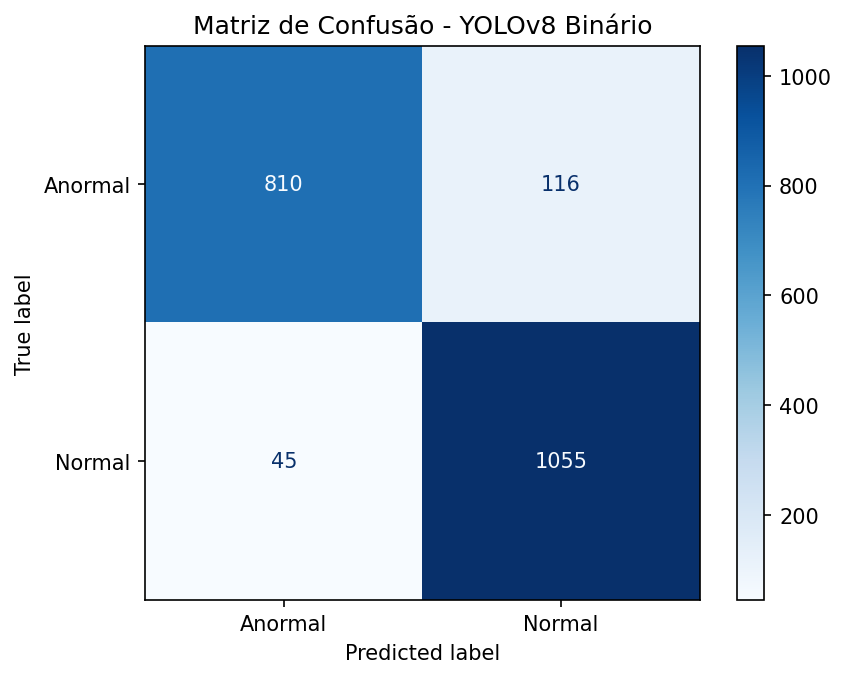
\includegraphics[width=0.55\textwidth]{yolo_binaria_matriz_confusao.png}
    \caption{Matriz de confusão visualizada --- classificação binária.}
    \label{fig:ybin_cm}
\end{figure}

\begin{figure}[H]
    \centering
    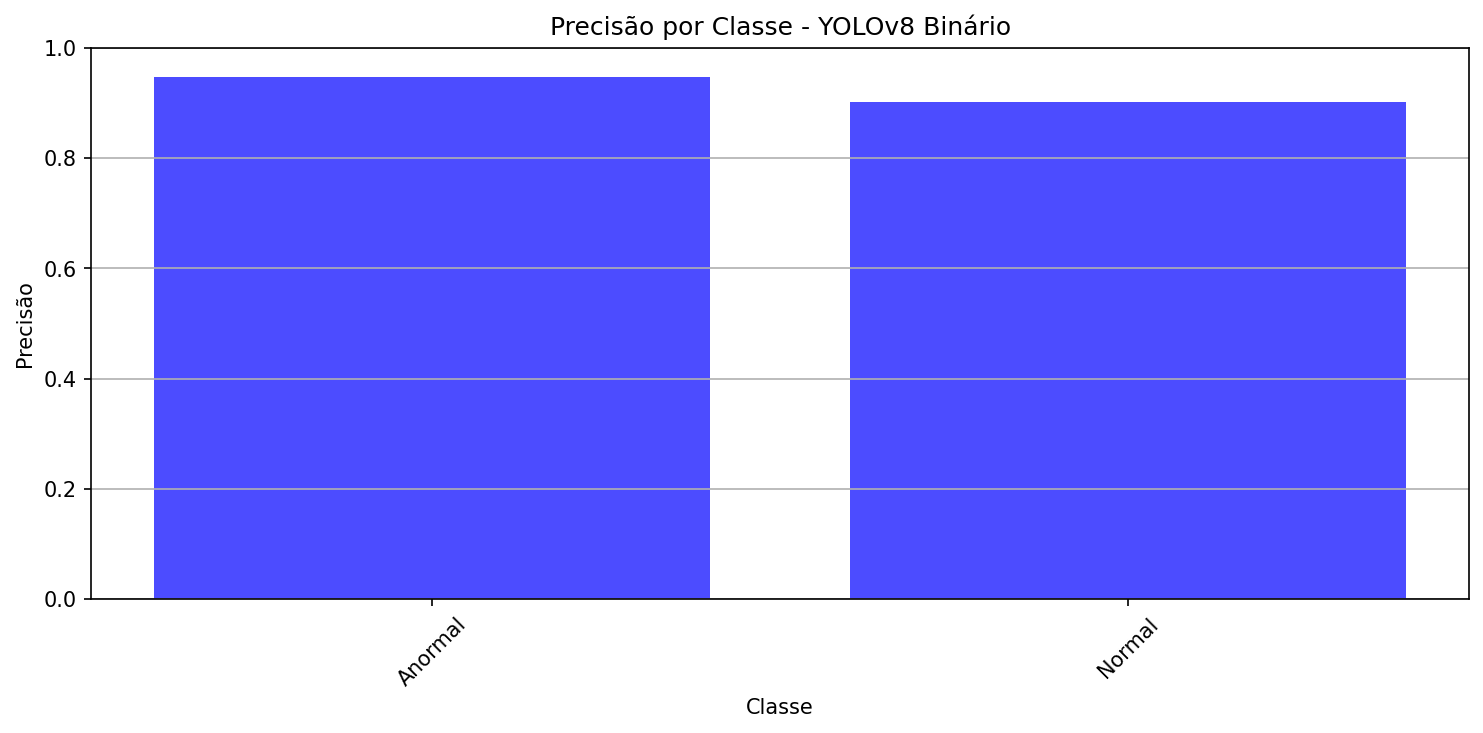
\includegraphics[width=0.9\textwidth]{yolo_binaria_precisao_classe.png}
    \caption{Precisão por classe --- classificação binária.}
    \label{fig:ybin_prec}
\end{figure}

\begin{figure}[H]
    \centering
    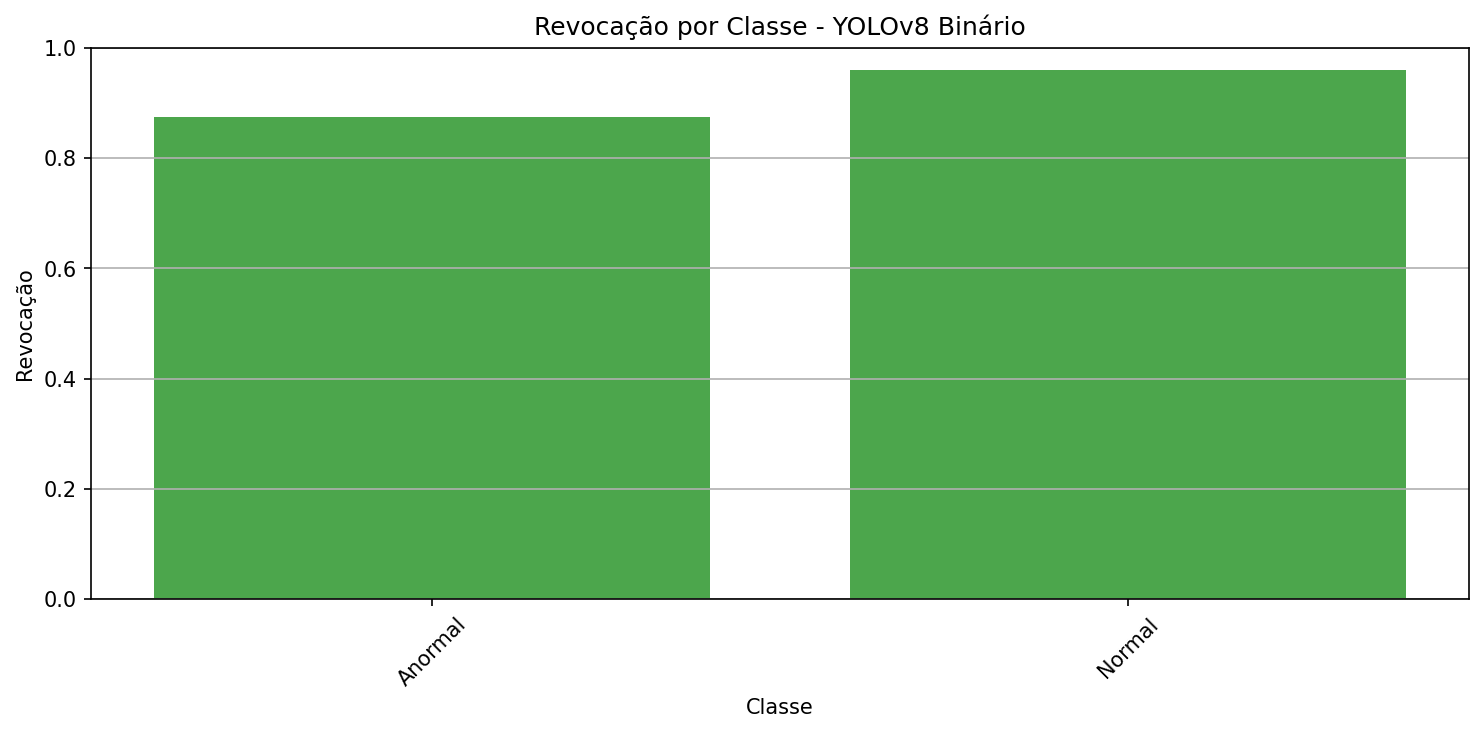
\includegraphics[width=0.9\textwidth]{yolo_binaria_revocacao_classe.png}
    \caption{Revocação por classe --- classificação binária.}
    \label{fig:ybin_rec}
\end{figure}

\begin{figure}[H]
    \centering
    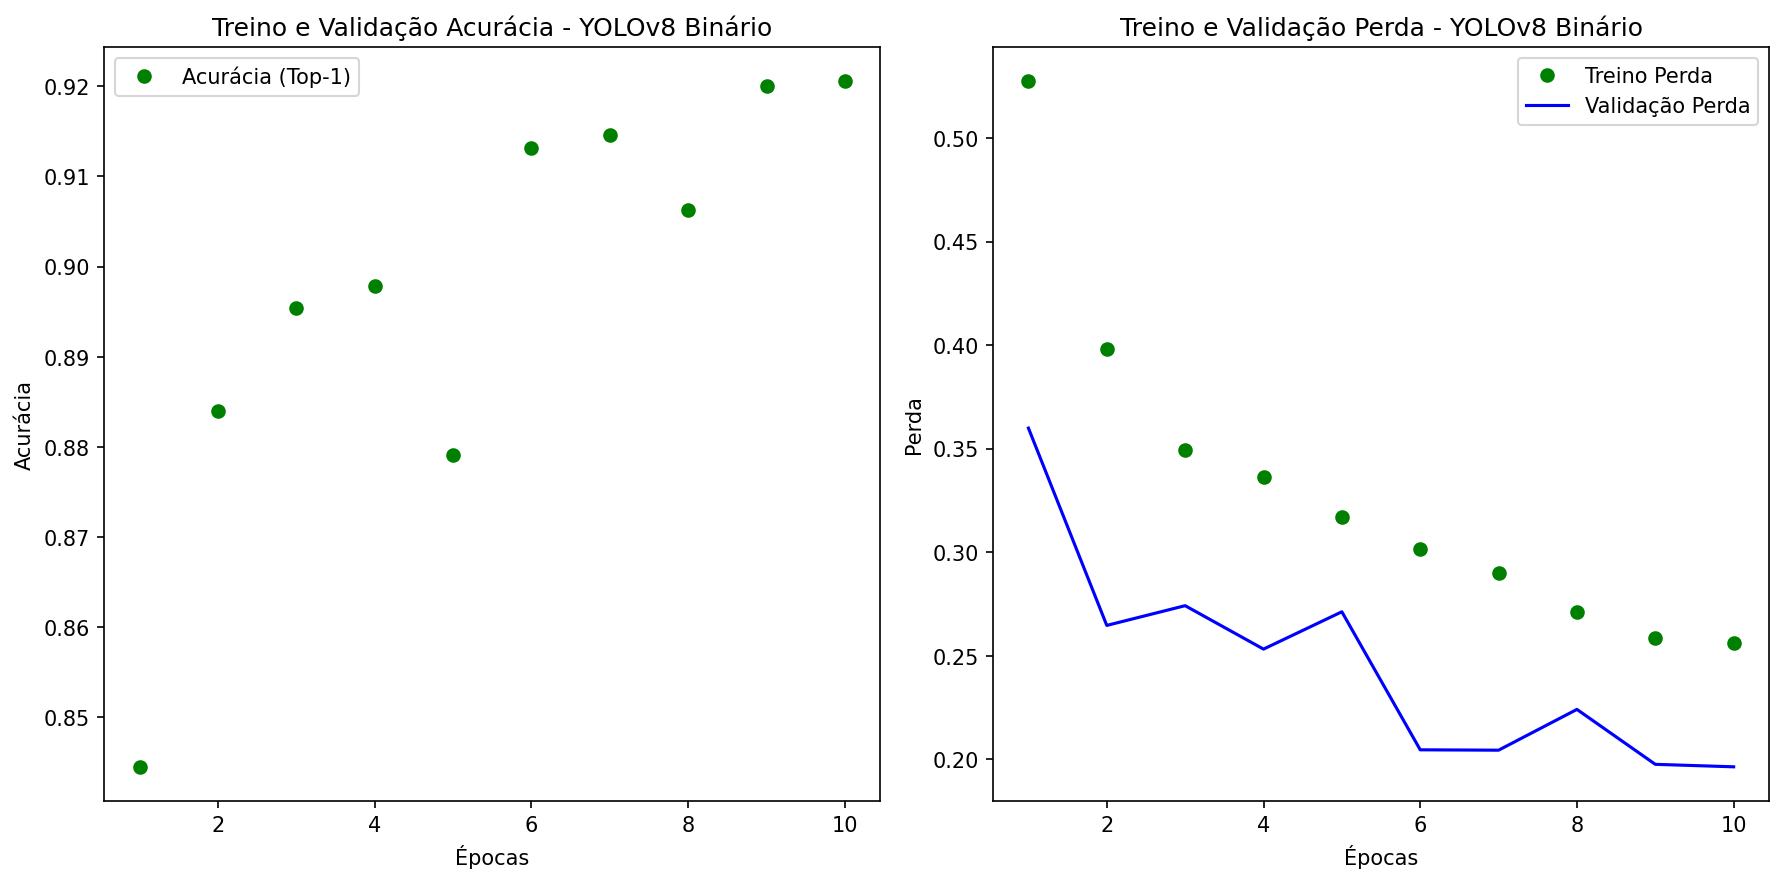
\includegraphics[width=0.9\textwidth]{yolo_binaria_convergencia.png}
    \caption{Convergência do treinamento --- classificação binária.}
    \label{fig:ybin_conv}
\end{figure}

\begin{figure}[H]
    \centering
    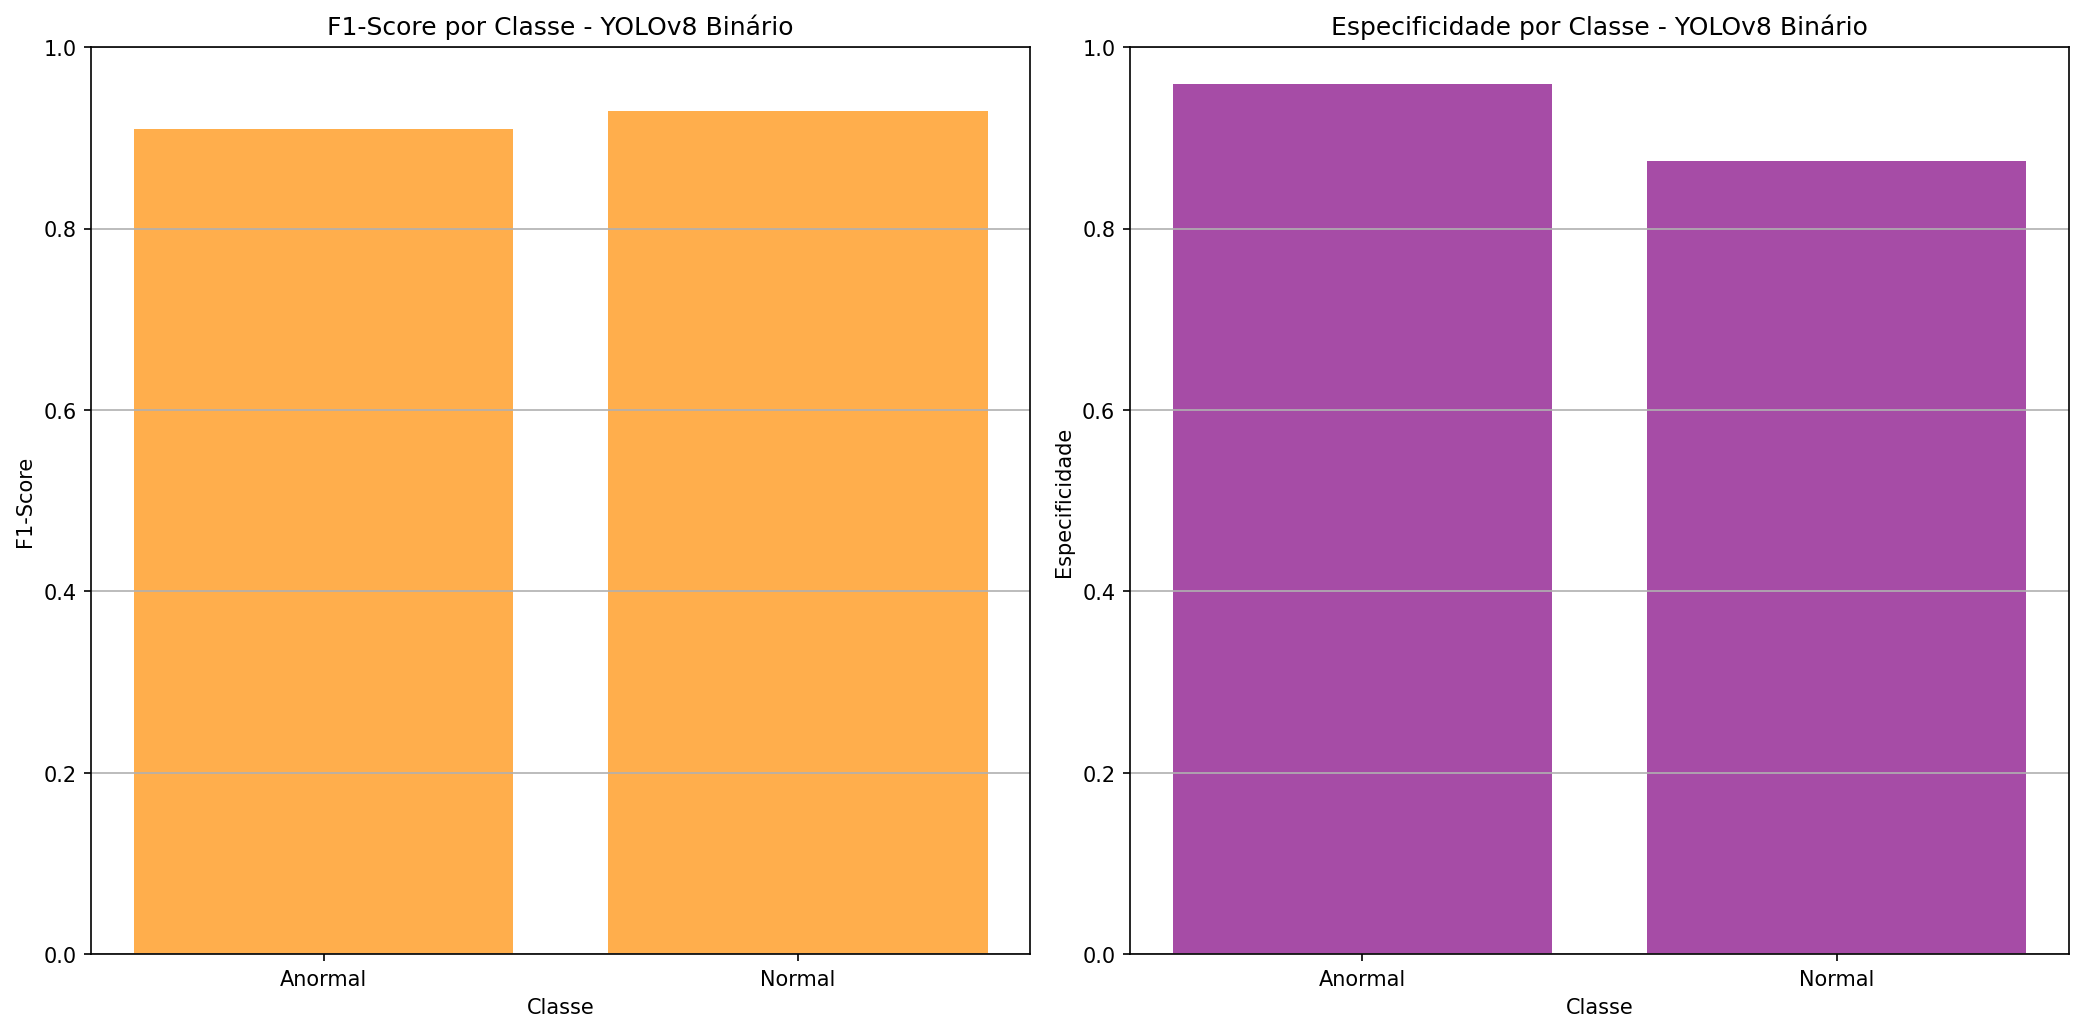
\includegraphics[width=0.9\textwidth]{yolo_binaria_f1_especificidade.png}
    \caption{F1-Score e especificidade por classe --- classificação binária.}
    \label{fig:ybin_f1spec}
\end{figure}

\subsection{Experimento 2: Classificação Multiclasse (6 Doenças)}

O segundo experimento classificou as células nas 6 categorias diagnósticas originais. A Tabela~\ref{tab:res_multi} apresentam as métricas gerais obtidas.

\begin{table}[H]
\centering
\caption{Resultados gerais do modelo YOLOv8 para classificação multiclasse.}
\label{tab:res_multi}
\begin{tabular}{lc}
\toprule
\textbf{Métrica} & \textbf{Valor} \\
\midrule
Acurácia              & 0,8238 \\
Precisão (weighted)   & 0,8103 \\
Revocação (weighted)  & 0,8238 \\
F1-Score (weighted)   & 0,8094 \\
\bottomrule
\end{tabular}
\end{table}

A acurácia de \textbf{82,38\%} na classificação em 6 classes é inferior à obtida no cenário binário (92,05\%), o que é esperado dado o aumento significativo da complexidade da tarefa e a semelhança morfológica entre determinadas classes de lesões.

A Tabela abaixo apresenta o relatório detalhado de classificação por classe:

\begin{table}[H]
\centering
\caption{Relatório detalhado por classe --- classificação multiclasse.}
\label{tab:detalhado_multi}
\begin{tabular}{lcccc}
\toprule
\textbf{Classe} & \textbf{Precisão} & \textbf{Revocação} & \textbf{F1-Score} & \textbf{Amostras} \\
\midrule
ASC-H     & 0,80 & 0,68 & 0,73 & 182 \\
ASC-US    & 0,52 & 0,26 & 0,35 & 124 \\
HSIL      & 0,81 & 0,87 & 0,84 & 336 \\
LSIL      & 0,77 & 0,57 & 0,66 & 260 \\
Negativa  & 0,85 & 0,96 & 0,91 & 1.100 \\
Carcinoma & 0,75 & 0,50 & 0,60 & 24 \\
\midrule
\textbf{Média (weighted)} & \textbf{0,81} & \textbf{0,82} & \textbf{0,81} & \textbf{2.026} \\
\bottomrule
\end{tabular}
\end{table}

A classe \textbf{Negativa} obteve o melhor desempenho (F1 = 0,91), o que é atribuído ao maior número de amostras disponíveis para treinamento (5.500 imagens). Em contrapartida, a classe \textbf{ASC-US} apresentou o pior desempenho (F1 = 0,35), com apenas 26\% de revocação, indicando que a maioria das amostras desta classe foram classificada incorretamente. A classe \textbf{Carcinoma}, apesar de possuir apenas 24 amostras no conjunto de validação, obteve precisão de 75\%, embora com revocação de apenas 50\%.

A Tabela abaixo apresenta a especificidade calculada por classe:

\begin{table}[H]
\centering
\caption{Especificidade por classe --- classificação multiclasse.}
\label{tab:especificidade}
\begin{tabular}{lc}
\toprule
\textbf{Classe} & \textbf{Especificidade} \\
\midrule
ASC-H     & 0,9837 \\
ASC-US    & 0,9848 \\
HSIL      & 0,9592 \\
LSIL      & 0,9757 \\
Negativa  & 0,8035 \\
Carcinoma & 0,9980 \\
\bottomrule
\end{tabular}
\end{table}

As especificidades são elevadas para todas as classes (acima de 0,95), com exceção da classe Negativa (0,8035). Isto indica que, quando o modelo prediz que uma amostra \textit{não} pertence a determinada classe, esta predição é altamente confiável. A menor especificidade da classe Negativa se deve ao fato de que várias amostras de outras classes são erroneamente classificadas como Negativa.

A Tabela abaixo apresenta a matriz de confusão completa:

\begin{table}[H]
\centering
\caption{Matriz de confusão --- classificação multiclasse.}
\label{tab:cm_multi}
\begin{tabular}{lcccccc}
\toprule
 & \textbf{ASC-H} & \textbf{ASC-US} & \textbf{HSIL} & \textbf{LSIL} & \textbf{Neg.} & \textbf{Carc.} \\
\midrule
\textbf{ASC-H}  & \textbf{123} & 1   & 31  & 9   & 18  & 0 \\
\textbf{ASC-US}  & 1   & \textbf{32}  & 5   & 12  & 73  & 1 \\
\textbf{HSIL}    & 12  & 1   & \textbf{293} & 9   & 18  & 3 \\
\textbf{LSIL}    & 6   & 19  & 15  & \textbf{148} & 72  & 0 \\
\textbf{Negativa}& 11  & 8   & 7   & 13  & \textbf{1061}& 0 \\
\textbf{Carc.}   & 0   & 0   & 11  & 0   & 1   & \textbf{12} \\
\bottomrule
\end{tabular}
\end{table}

A análise da matriz de confusão revela que as confusões mais frequentes ocorre entre:
\begin{itemize}
    \item \textbf{ASC-US $\rightarrow$ Negativa:} 73 amostras de ASC-US foram classificadas como Negativa, correspondendo a 58,9\% das amostras desta classe. Isto é clinicamente preocupante, pois representa falsos negativos.
    \item \textbf{LSIL $\rightarrow$ Negativa:} 72 amostras de LSIL foram incorretamente atribuídas à classe Negativa (27,7\%).
    \item \textbf{ASC-H $\rightarrow$ HSIL:} 31 amostras de ASC-H foram classificadas como HSIL, o que é compreensível dada a semelhança morfológica entre estas lesões.
\end{itemize}

\begin{figure}[H]
    \centering
    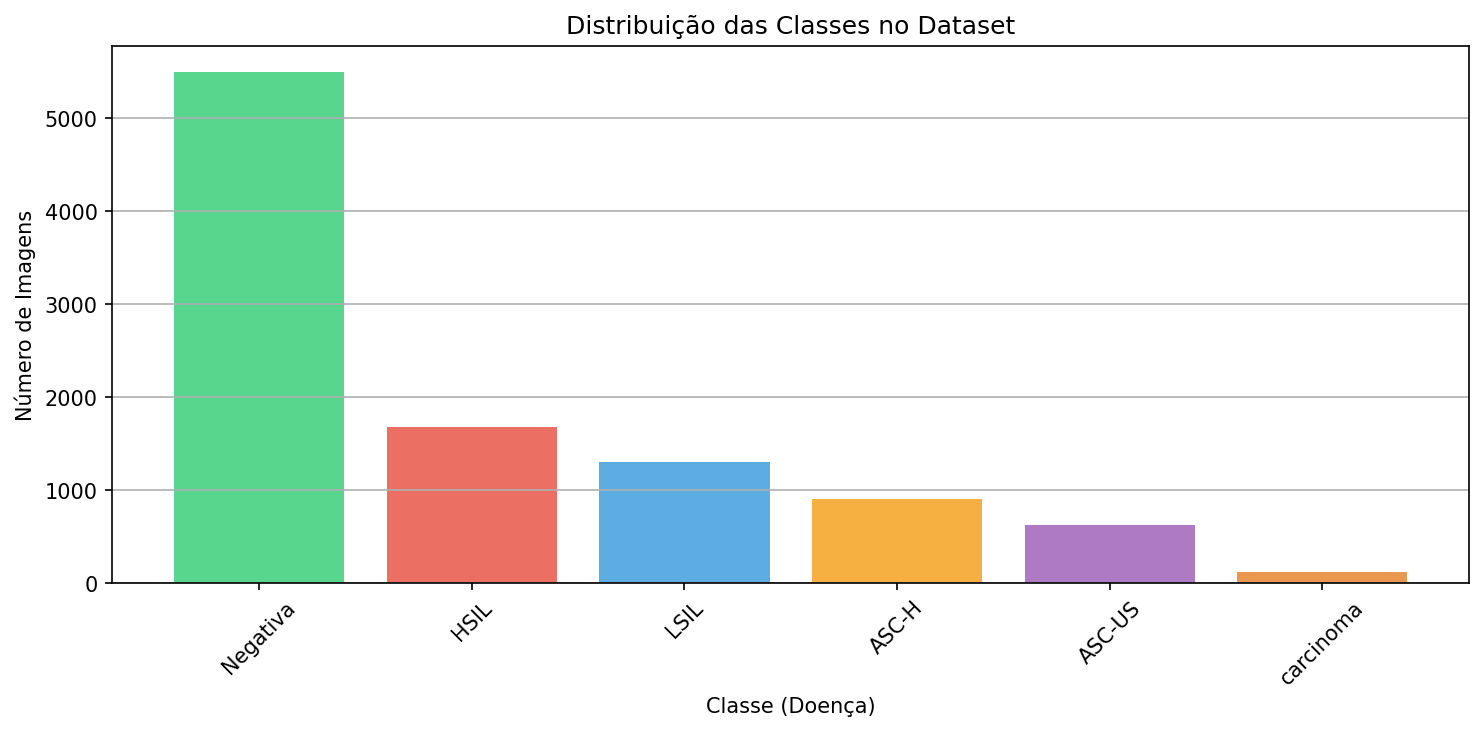
\includegraphics[width=0.9\textwidth]{yolo_multiclasse_distribuicao_classes.png}
    \caption{Distribuição das classes no dataset de treinamento.}
    \label{fig:ymulti_dist}
\end{figure}

\begin{figure}[H]
    \centering
    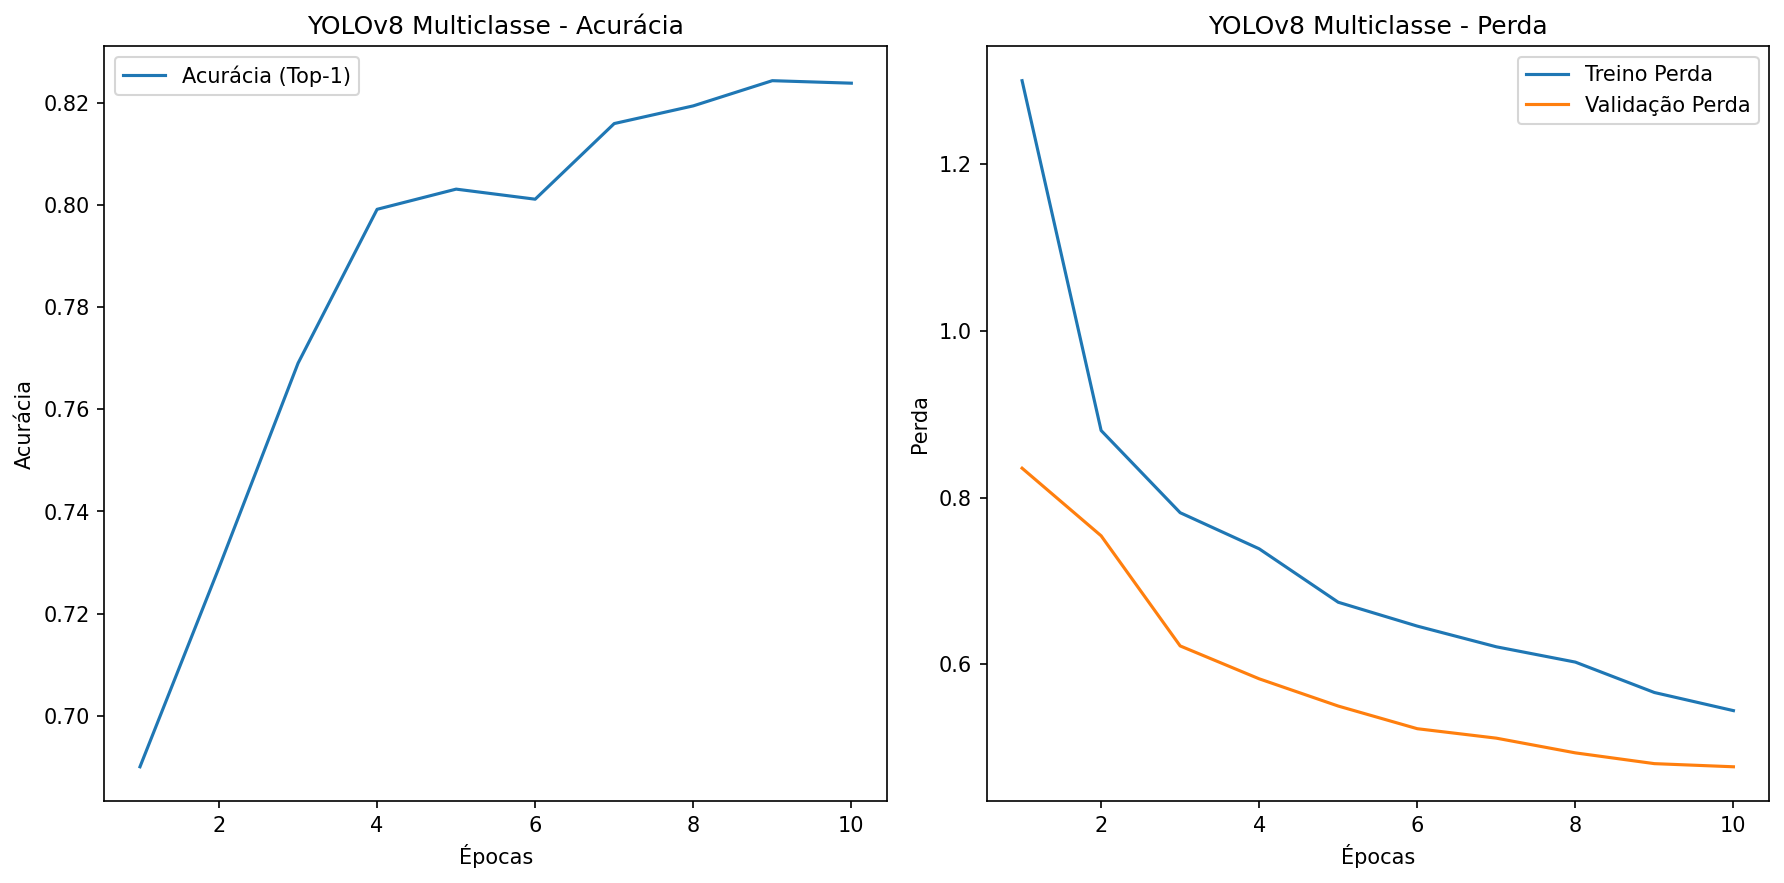
\includegraphics[width=0.9\textwidth]{yolo_multiclasse_acuracia_perda.png}
    \caption{Curvas de acurácia e perda ao longo das épocas --- classificação multiclasse.}
    \label{fig:ymulti_acc_loss}
\end{figure}

\begin{figure}[H]
    \centering
    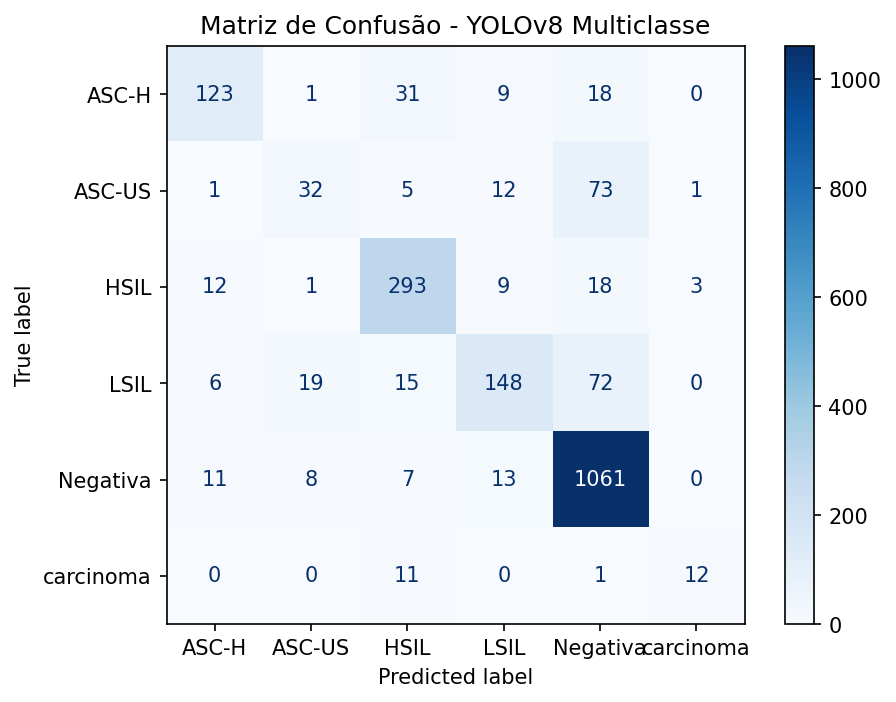
\includegraphics[width=0.55\textwidth]{yolo_multiclasse_matriz_confusao.png}
    \caption{Matriz de confusão visualizada --- classificação multiclasse.}
    \label{fig:ymulti_cm}
\end{figure}

\begin{figure}[H]
    \centering
    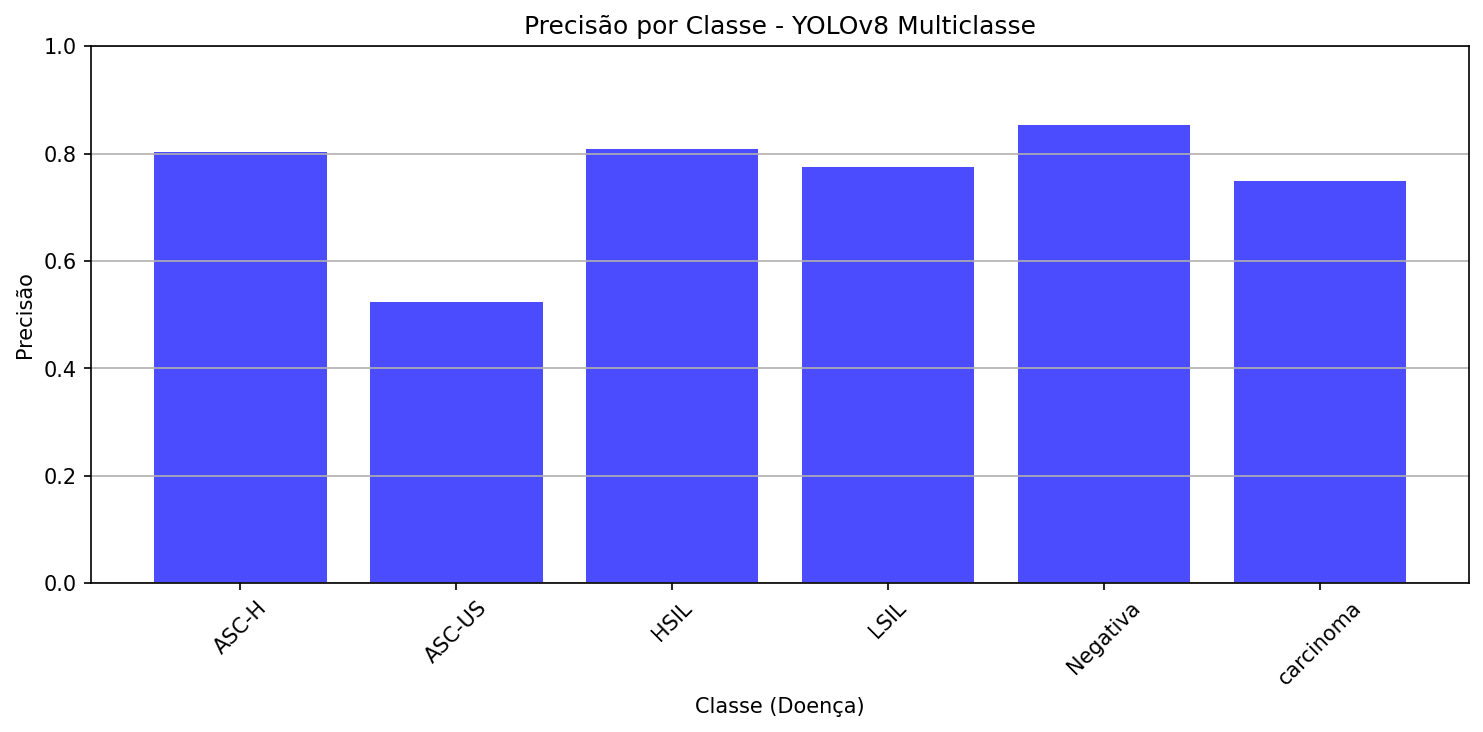
\includegraphics[width=0.9\textwidth]{yolo_multiclasse_precisao_classe.png}
    \caption{Precisão por classe --- classificação multiclasse.}
    \label{fig:ymulti_prec}
\end{figure}

\begin{figure}[H]
    \centering
    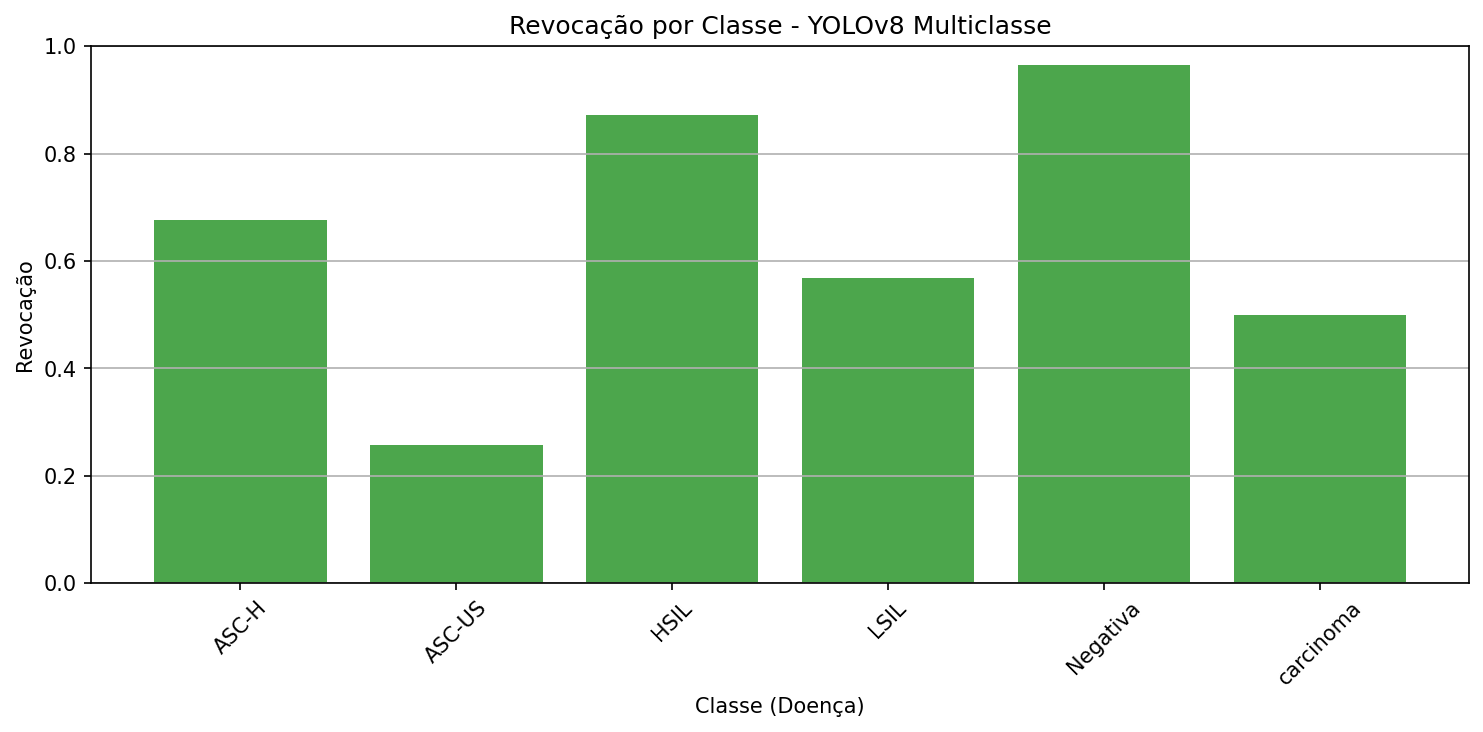
\includegraphics[width=0.9\textwidth]{yolo_multiclasse_revocacao_classe.png}
    \caption{Revocação por classe --- classificação multiclasse.}
    \label{fig:ymulti_rec}
\end{figure}

\begin{figure}[H]
    \centering
    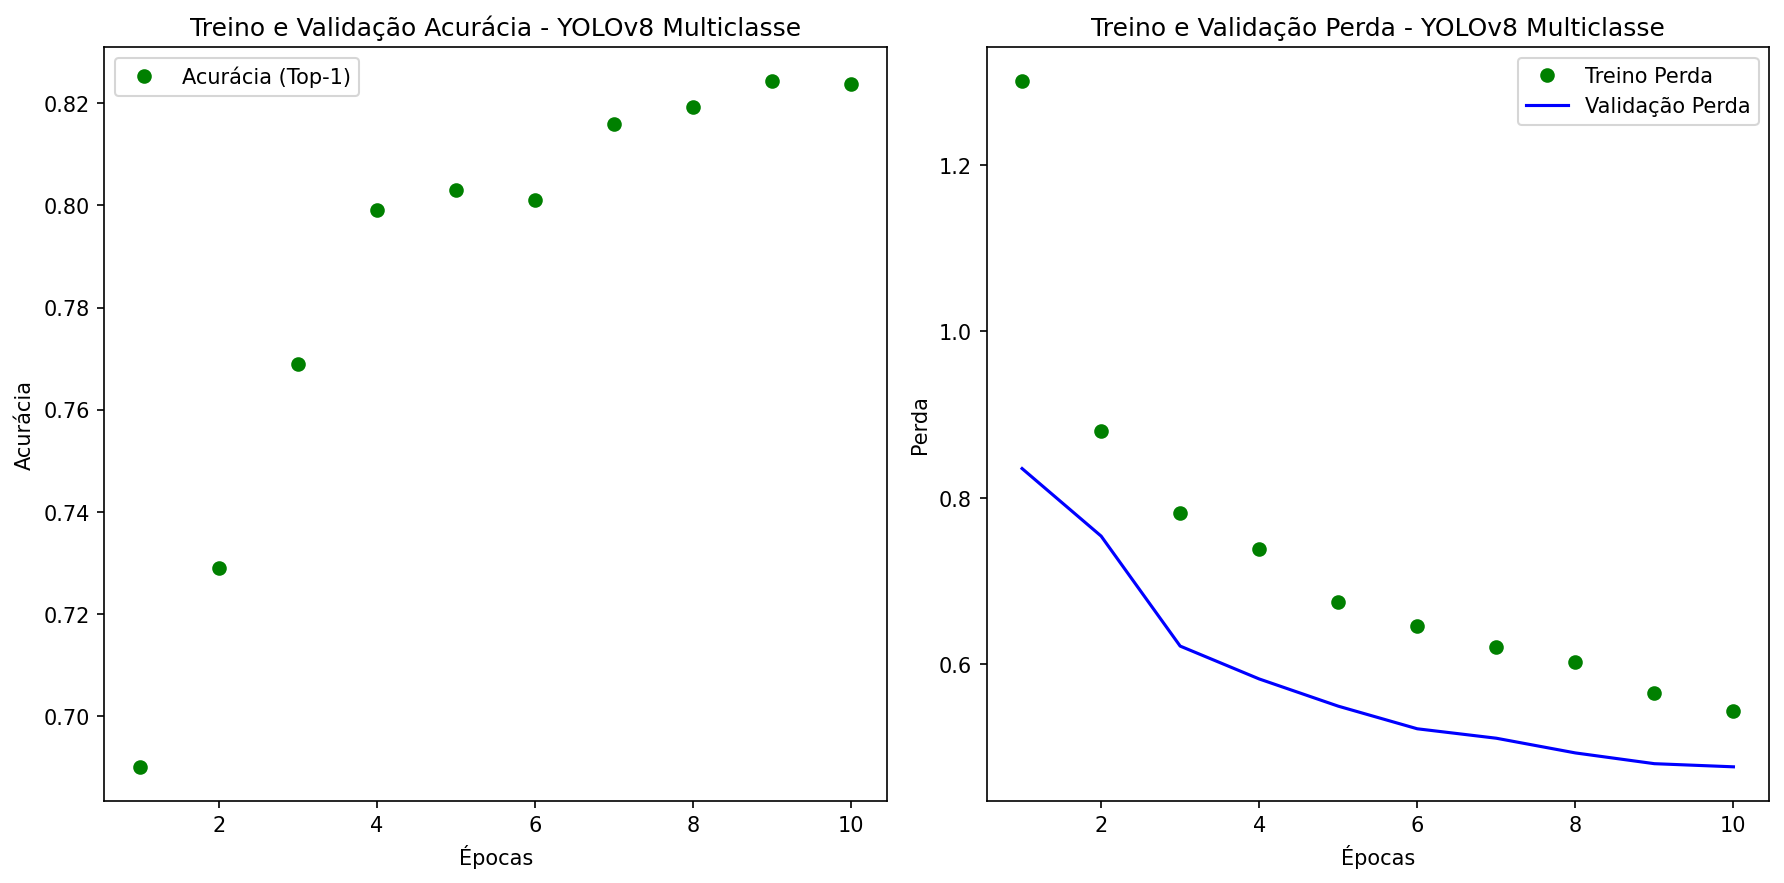
\includegraphics[width=0.9\textwidth]{yolo_multiclasse_convergencia.png}
    \caption{Convergência do treinamento --- classificação multiclasse.}
    \label{fig:ymulti_conv}
\end{figure}

\begin{figure}[H]
    \centering
    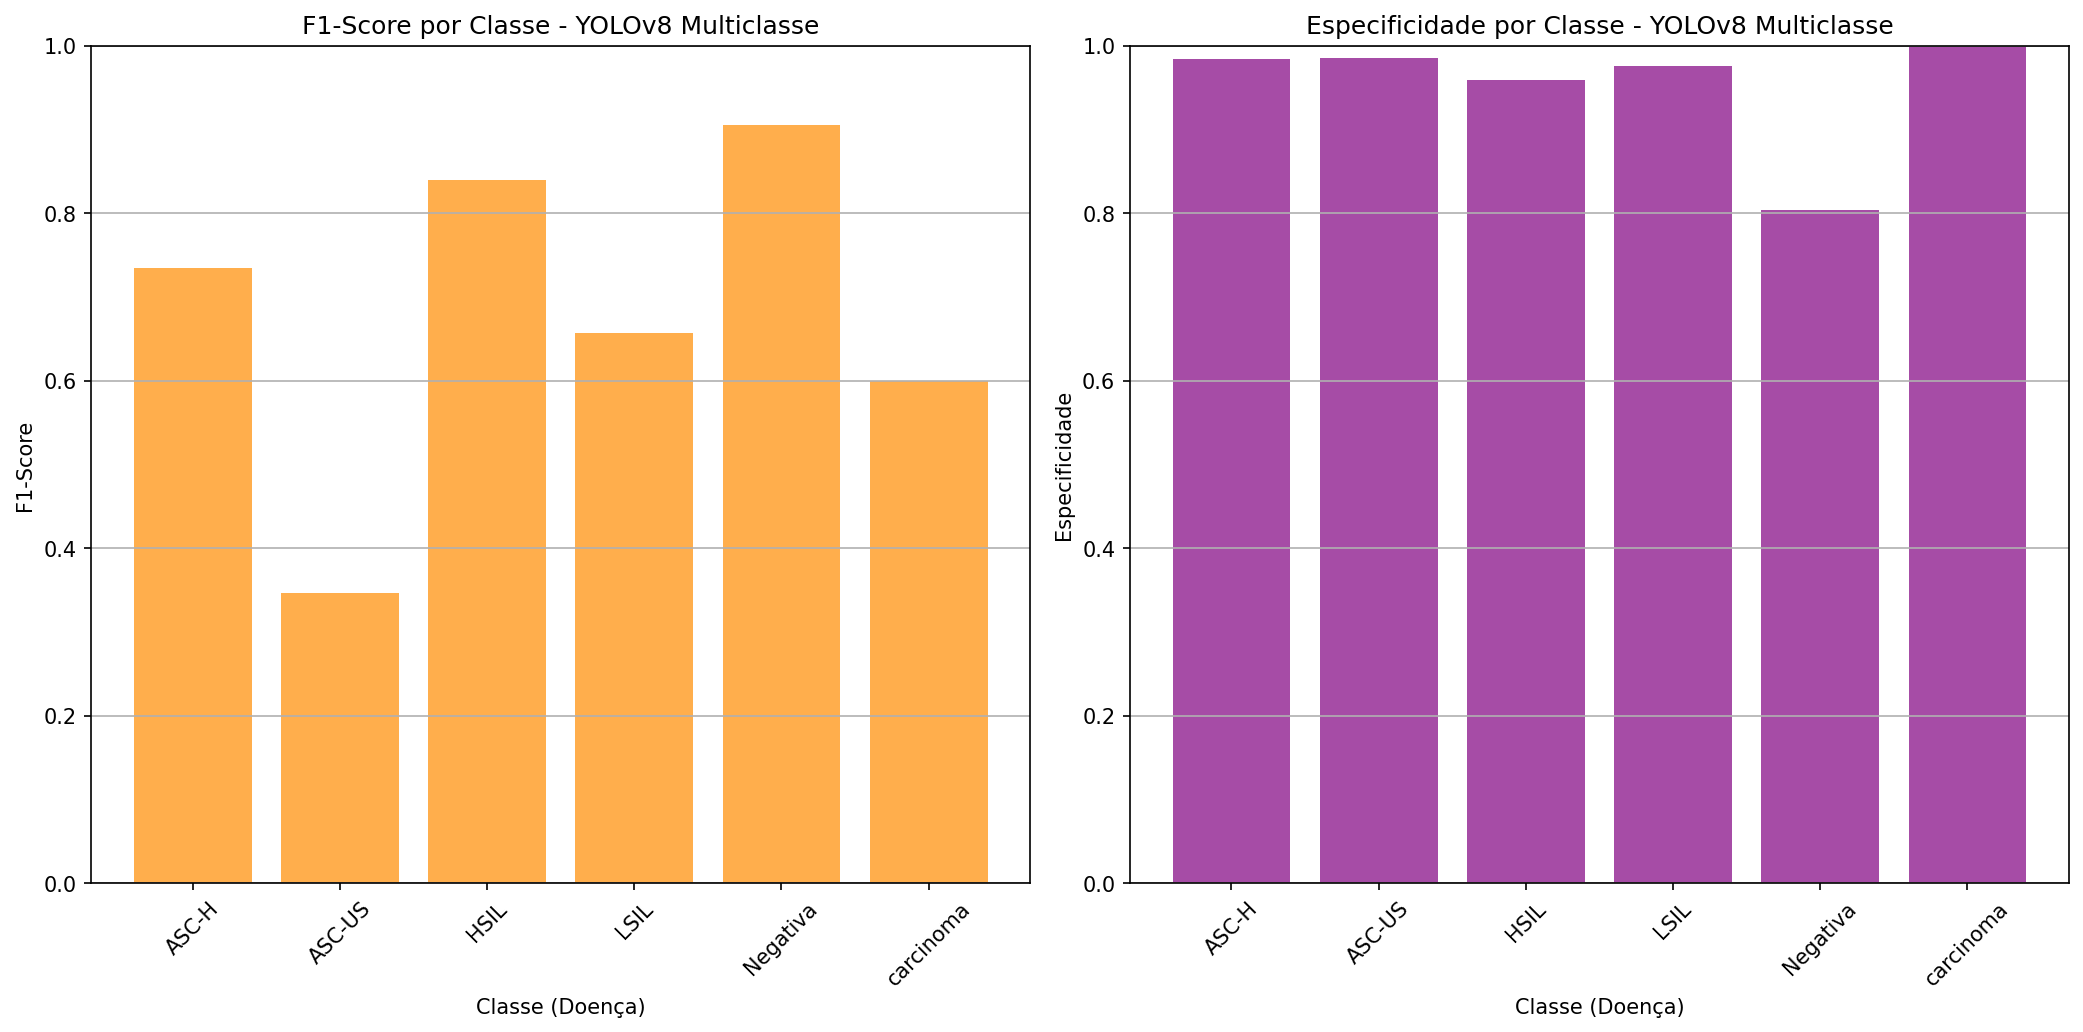
\includegraphics[width=0.9\textwidth]{yolo_multiclasse_f1_especificidade.png}
    \caption{F1-Score e especificidade por classe --- classificação multiclasse.}
    \label{fig:ymulti_f1spec}
\end{figure}

\begin{figure}[H]
    \centering
    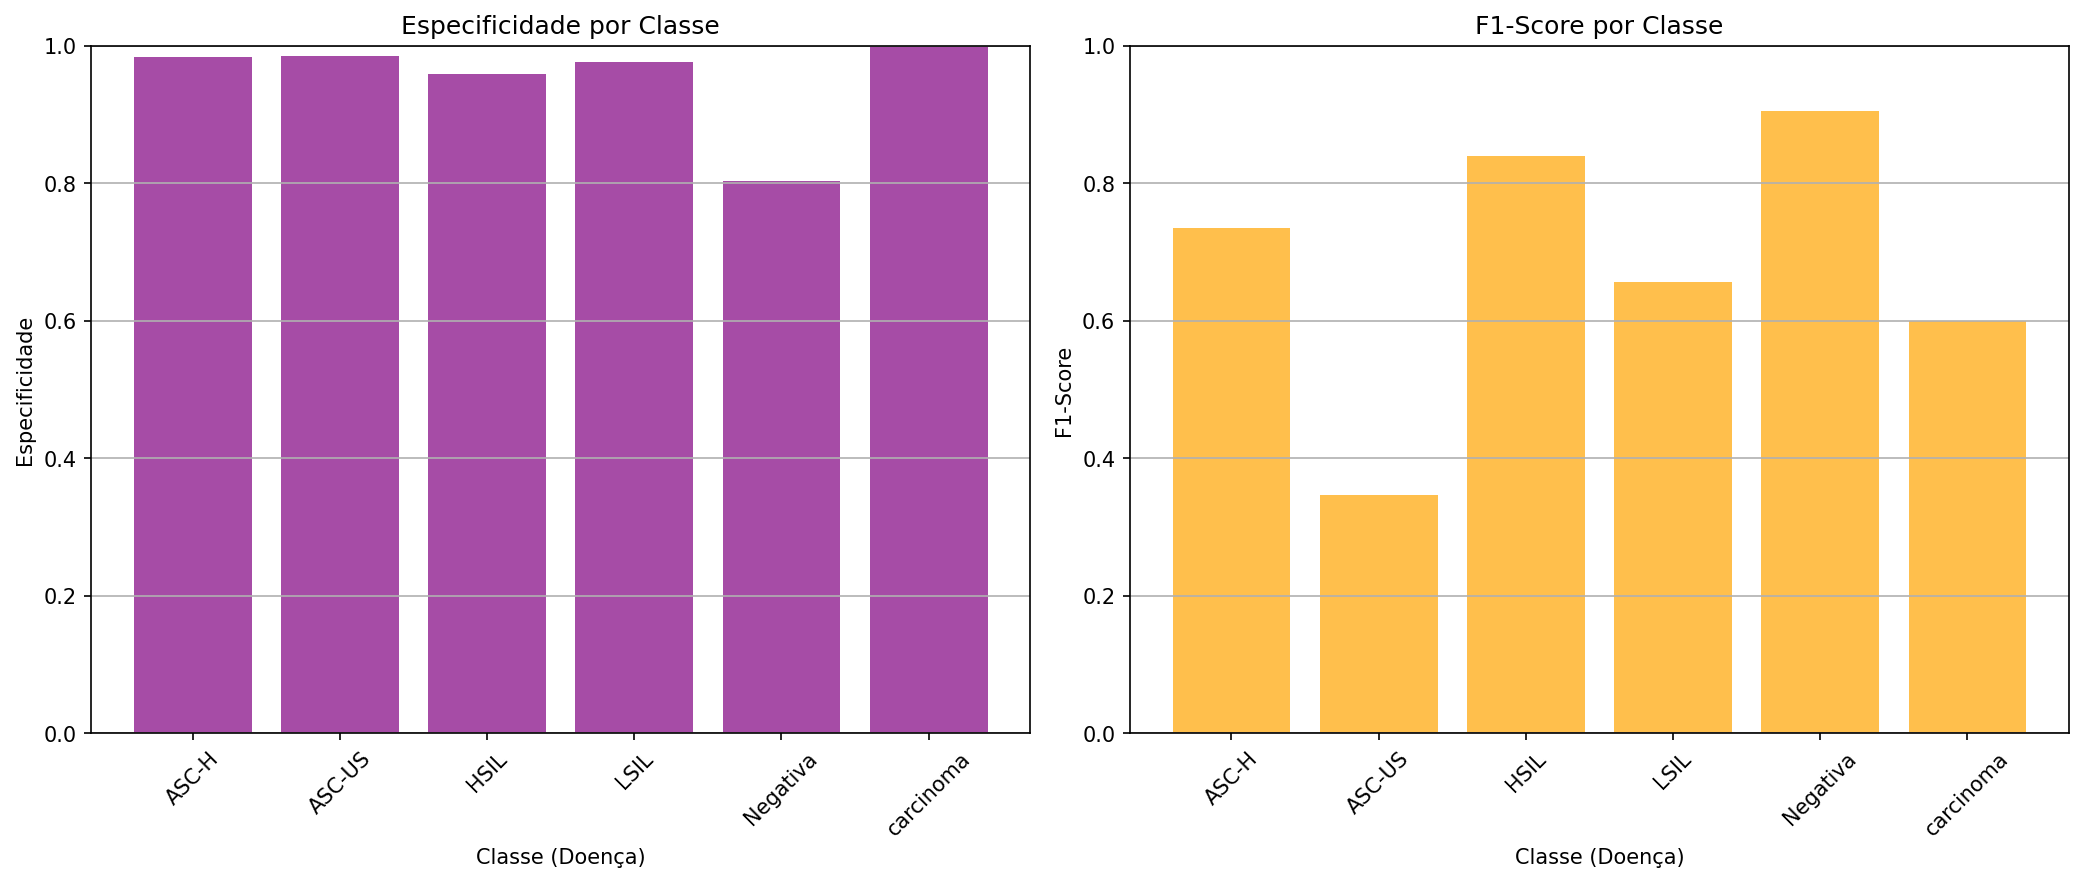
\includegraphics[width=0.9\textwidth]{yolo_multiclasse_especificidade_f1_classe.png}
    \caption{Especificidade e F1-Score por classe (comparativo) --- classificação multiclasse.}
    \label{fig:ymulti_spec_f1}
\end{figure}

\subsection{Comparação entre os Experimentos}

A Tabela abaixo sintetiza a comparação entre as duas abordagens experimentais.

\begin{table}[H]
\centering
\caption{Comparação dos resultados entre classificação binária e multiclasse.}
\label{tab:comparacao}
\begin{tabular}{lcc}
\toprule
\textbf{Métrica} & \textbf{Binário (2 classes)} & \textbf{Multiclasse (6 classes)} \\
\midrule
Acurácia              & 0,9205 & 0,8238 \\
Precisão (weighted)   & 0,9222 & 0,8103 \\
Revocação (weighted)  & 0,9205 & 0,8238 \\
F1-Score (weighted)   & 0,9202 & 0,8094 \\
Especificidade        & 0,8747 & 0,9508 (média) \\
\bottomrule
\end{tabular}
\end{table}

Conforme esperado, o modelo binário apresenta resultados superiores em acurácia, precisão, revocação e F1-Score, uma vez que a tarefa de distinguir entre apenas duas classes é inerentemente mais simples. Entretanto, a classificação multiclasse fornece informação clínica substancialmente mais relevantes, possibilitando a identificação do tipo específico da lesão.

% ============================================================
\section{Discussão}
% ============================================================

\subsection{Desempenho do YOLOv8 como Classificador}

Os resultados demonstra que o YOLOv8 no modo \textit{classify} é capaz de alcançar desempenho satisfatório na classificação de células cervicais, mesmo com imagens de baixa resolução ($50 \times 50$ pixels) e um dataset moderadamente desbalanceado. A utilização de \textit{transfer learning} a partir de pesos pré-treinados no ImageNet contribuiu significativamente para a convergência do modelo em apenas 10 épocas.

\subsection{Impacto do Desbalanceamento}

O desbalanceamento entre as classes apresentou impacto direto nos resultados, especialmente na classificação multiclasse. As classes com menor representação (ASC-US com 620 amostras e Carcinoma com 120 amostras) obtiveram revocação significativamente inferior às classes majoritárias. A classe ASC-US, com F1-Score de apenas 0,35, ilustra claramente este efeito: com apenas 124 amostras no conjunto de validação, o modelo não consegue aprender adequadamente os padrões discriminativos desta classe.

\subsection{Confusões Clinicamente Relevantes}

A análise da matriz de confusão multiclasse revela padrões de erro que possuem implicações clínicas importante:

\begin{itemize}
    \item A confusão frequente entre ASC-US e Negativa (58,9\% de falsos negativos) é a mais preocupante, pois implica que lesões de significado indeterminado podem não ser detectada pelo sistema.
    \item A confusão entre ASC-H e HSIL é menos crítica do ponto de vista clínico, pois ambas são lesões que requerem acompanhamento médico.
    \item A classe Carcinoma, embora com poucos exemplos, não foi confundida com a classe Negativa, o que é positivo para a triagem de casos graves.
\end{itemize}

\subsection{Limitações}

As principal limitações identificadas neste trabalho incluem:

\begin{itemize}
    \item A resolução das imagens ($50 \times 50$ pixels) é relativamente baixa para a análise citológica, podendo limitar a capacidade do modelo de capturar detalhes morfológicos sutis.
    \item O número de épocas (10) pode ser insuficiente para a convergência completa do modelo, especialmente no cenário multiclasse.
    \item O desbalanceamento severo entre as classes não foi tratado com técnicas específicas como \textit{oversampling} ou pesos de classe.
\end{itemize}

% ============================================================
\section{Implementação}
% ============================================================

Todo o código foram desenvolvido integralmente pelo aluno, sem utilização de aplicações ou \textit{pipelines} prontos de classificação. A implementação consiste em dois scripts Python independentes, conforme descrito na Tabela~\ref{tab:arquivos}.

\begin{table}[H]
\centering
\caption{Descrição dos arquivos de implementação.}
\label{tab:arquivos}
\begin{tabular}{lp{9.5cm}}
\toprule
\textbf{Arquivo} & \textbf{Descrição} \\
\midrule
\texttt{yolo\_binario.py} & Classificação binária (Normal vs. Anormal) utilizando YOLOv8. Inclui reorganização dos dados, treinamento com \textit{transfer learning}, avaliação de métricas e geração de 6 gráficos salvos em PNG. \\
\addlinespace
\texttt{yolo\_doencas.py} & Classificação multiclasse (6 doenças) utilizando YOLOv8. Inclui reorganização com 6 classes, treinamento, relatório detalhado por classe, especificidade por classe e geração de 8 gráficos. \\
\bottomrule
\end{tabular}
\end{table}

\subsection{Bibliotecas Utilizadas}

\begin{table}[H]
\centering
\caption{Bibliotecas e suas respectivas funções no projeto.}
\label{tab:bibliotecas}
\begin{tabular}{ll}
\toprule
\textbf{Biblioteca} & \textbf{Utilização} \\
\midrule
Ultralytics (YOLOv8) & Treinamento e inferência do modelo de classificação \\
scikit-learn         & Métricas de avaliação e divisão estratificada dos dados \\
NumPy                & Manipulação de arrays numéricos \\
Pandas               & Leitura do histórico de treinamento (CSV) \\
Matplotlib           & Geração de gráficos e visualizações \\
shutil               & Cópia de arquivos para reorganização do dataset \\
\bottomrule
\end{tabular}
\end{table}

% ============================================================
\section{Conclusão}
% ============================================================

O presente trabalho demonstrou a viabilidade da utilização do YOLOv8 no modo \textit{classify} para a classificação automática de células cervicais provenientes de exames de Papanicolaou. Foram conduzidos dois experimentos complementares:

\begin{enumerate}
    \item Uma \textbf{classificação binária} (Normal vs. Anormal) que alcançou acurácia de 92,05\%, F1-Score de 0,92 e especificidade de 87,47\%, demonstrando eficácia como ferramenta de triagem inicial.

    \item Uma \textbf{classificação multiclasse} em 6 categorias diagnósticas que obteve acurácia de 82,38\% e F1-Score ponderado de 0,81, com destaque para o desempenho da classe HSIL (F1 = 0,84) e Negativa (F1 = 0,91), e com desempenho inferior para ASC-US (F1 = 0,35) devido ao desbalanceamento e semelhança morfológica.
\end{enumerate}

A variação do hiperparâmetro principal --- o número de classes de saída (2 vs. 6) --- produziu diferenças significativas nos resultados, evidenciando o \textit{trade-off} entre granularidade diagnóstica e desempenho do modelo. O uso de \textit{transfer learning} a partir de pesos pré-treinados no ImageNet mostrou-se eficaz para a convergência rápida do modelo mesmo com um dataset de tamanho moderado.

Como trabalhos futuros, sugere-se: (i) a aplicação de técnicas de \textit{data augmentation} para mitigar o desbalanceamento; (ii) o uso de pesos de classe durante o treinamento; (iii) o aumento da resolução das imagens de entrada; (iv) a exploração de variantes maiores do YOLOv8 (small, medium, large) para avaliar o impacto da capacidade do modelo; e (v) o aumento do número de épocas de treinamento.

\end{document}
